\documentclass[12pt]{article}
\usepackage[utf8]{inputenc}
\usepackage[T2A]{fontenc}
\usepackage[russian]{babel}
\usepackage{amsmath}
\usepackage{amssymb}
\usepackage{dsfont}
\usepackage[dvipsnames]{xcolor}
\usepackage{setspace}
\usepackage{multirow}
\usepackage[a4paper, outer=1.5cm, inner=1.5cm, top=1cm, bottom=1cm]{geometry}
\usepackage{graphicx}
\usepackage{skull}
\usepackage{wasysym}
\usepackage{float}
\graphicspath{{.images/}}
\usepackage{hyperref}
\hypersetup{colorlinks=true, linkcolor=blue, filecolor=magenta, urlcolor=cyan}
\usepackage[firstpage]{draftwatermark}
\SetWatermarkText{
    $\qquad\qquad\qquad\qquad\qquad$\parbox{7cm}{\begin{center}
    
\includegraphics[width = 0.08\textwidth]{lion-logo.png}\bigskip\\~\bigskip\\~\vspace{-24mm}\\~\end{center}}
}
\SetWatermarkAngle{0}
\SetWatermarkScale{1.5}
\usepackage{etoolbox}

\newtoggle{ifsolved}
\newtoggle{needhelp}
\newcounter{num}
\setcounter{num}{1}

\newcommand{\newnum}{\par\textbf{\textnumero\arabic{num}}\stepcounter{num}}
\newcommand{\sol}{\vspace{3mm}\par\textbf{Решение: }}
\newcommand{\ans}{\vspace{3mm}\par\textbf{Ответ: }}
\newcommand{\hint}{\vspace{3mm}\par\textbf{Подсказка: }}
\newcommand{\mode}[1]{
\ifstrequal{#1}{0}{\togglefalse{ifsolved}\togglefalse{needhelp}}{\ifstrequal{#1}{1}{\togglefalse{ifsolved}\toggletrue{needhelp}}{\ifstrequal{#1}{2}{\toggletrue{ifsolved}\togglefalse{needhelp}}{\toggletrue{ifsolved}\toggletrue{needhelp}}}}} %if 0 - if 1 - if 2 - else
%\newenvironment{problem}[8]{%#1, #2, #3
%\parbox{\linewidth}{\vspace{4mm}\ifstrequal{#4}{(лёгкая)}{\newnum\textbf{.}}{\newnum\textbf{*.} } \\ #5}
%\iftoggle{ifsolved}{\sol #6}{}
%\iftoggle{ifsolved}{\ans #7}{}
%\iftoggle{needhelp}{\hint #8}{}}

\newenvironment{problem}[8]{%#1, #2, #3
\parbox{\linewidth}{\vspace{5mm}\ifstrequal{#4}{(лёгкая)}{\newnum\textbf{.}}{\newnum\textbf{*.} } \\ #5}
\iftoggle{ifsolved}{\sol #6}{}

\iftoggle{ifsolved}{\parbox{\linewidth}{\ans #7}}{}
\iftoggle{needhelp}{\parbox{\linewidth}{\hint #8}}{}}

\newenvironment{mylist} %custom list
{ \begin{itemize}
    \setlength{\itemsep}{0pt}
    \setlength{\parskip}{0pt}
    \setlength{\parsep}{0pt}     }
{ \end{itemize}                  }

\newenvironment{homeass}[1]{\vspace*{-1.5cm}
\iftoggle{ifsolved}{
    \section*{\center{Решение домашнего задания к #1.}}
}{
    \section*{\center{\textcolor{Sepia}{Домашнее задание к #1}}}
} \vspace{7mm}\large}

\parindent=0pt
\pagestyle{empty}
%$\!$[\arabic{class}.\arabic{num}]
%\ifnumcomp{\value{counter}}{>}{1}{true}{false}
%\definecolor{Gray}{gray}{0.9}
%\definecolor{mypink}{RGB}{219, 48, 122}
%\newcolumntype{g}{>{\columncolor{Gray}}p{2.8cm}}

\begin{document}
\large
\mode{7}
%0 for problems without hints
%1 for problems + hints
%2 for problems + solutions + answers
%else: show all

{\centering\section*{СПИСОК ЗАДАЧ}}

{\centering\subsection*{\smallskip\\\textcolor{green}{\textbf{Полезные вещи, которые можно и нужно копипастить:}}}}

\subsection*{\textcolor{Emerald}{\textbf{Полезные шпаргалки по LaTeXу:}}}

\textbf{Пример вставки рисунка:}

\begin{minipage}{\linewidth}
    \begin{minipage}{0.54\linewidth}
    см. рисунок справа\\
    Текст к собственно пикче, примерно всегда это либо развёрнутое описание, либо большая часть решения задачи --- стремимся экономить пространство, если это можно сделать.
    \end{minipage}
    \hspace{0.05\linewidth}
    \begin{minipage}{0.4\linewidth}
    \begin{figure}[H] 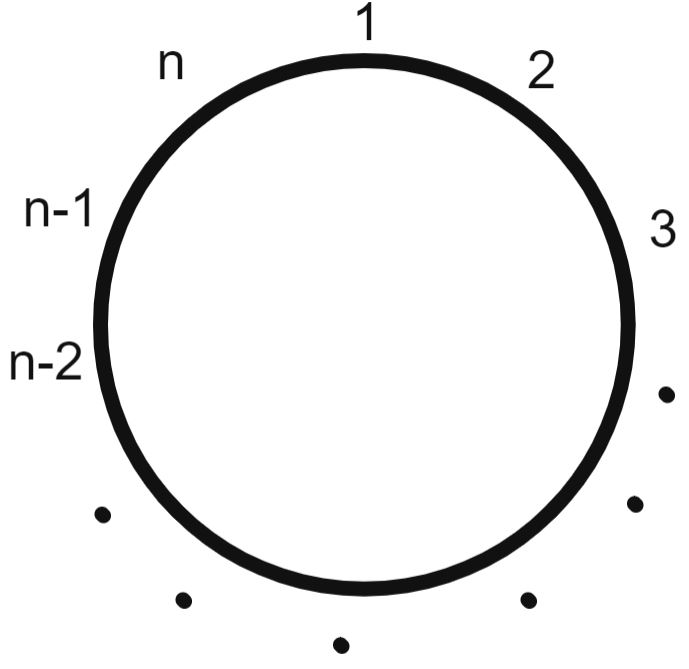
\includegraphics[width=\linewidth]{sol3} %тут поменять имя пикчи
    \end{figure}
    \end{minipage}
\end{minipage}

\textbf{Дефолтные математические знаки и символы:}\\
$\geqslant$,
$\leqslant$,
$a^{b}$,
$x_{i}$,
$\sqrt{a}$,
$\frac{a}{b}$,
$\displaystyle \frac{a}{b}$,
$\cdot$
$\;\Rightarrow\;$,
$\;\Leftrightarrow\;$,
$1{,}2$.
О промежутках:
$a\!b$,
$a\,b$,
$a\:b$,
$a\;b$,
$a\quad b$.

\textbf{Стандартные система и совокупность уравнений / неравенств:}\\
$\left\{
\begin{aligned}
f(x) &= 0 \\
g(x) &= 1
\end{aligned}\right.$

$\left[\begin{aligned}
&\left\{\begin{aligned}
f(x) &\geqslant a \\
g(x) &= b
\end{aligned}\right.\\
&\left\{\begin{aligned}
f(x) &< a \\
g(x) &= -b
\end{aligned}\right.
\end{aligned}\right.$

\subsection*{\textcolor{Emerald}{\textbf{Не математическое, но полезное:}}}
% комментарий в любом месте документа, который нигде не будет видно. Можно использовать для написания заметок-вопросов по задачам
\textbf{Пример таблицы:}

\begin{tabular}{|c|c|c|}
\hline
    $a$ & $b$ & текст
\\\hline
    $c$ & $d$ & мораль
\\\hline
\end{tabular}\\

\textbf{Отступы:} между\smallskip\\ строками\medskip\\ \textbf{Тире} --- это три дефиса.\\
\textbf{Списки:}
\begin{mylist}
\item [$\bullet$] это был пункт а
\item [2)] а это уже пункт номер 2 с изменённым заголовком
\end{mylist}

\subsection*{\textcolor{Emerald}{\textbf{Всё, неупомянутое выше (или если просто что-то не так):}}}
\begin{mylist}
\item [$\bullet$] Решение отдельных вопросов касательно ТеХа нужно искать в \href{https://www.mccme.ru/free-books/llang/newllang.pdf}{Львовском}.

\item [$\bullet$] Найти произвольный символ, который нужен, можно в \href{http://detexify.kirelabs.org/classify.html}{Detexify}.

\item [$\bullet$] Если возникли сомнения при решении, ответ практически ко всем задачам можно проверить с помощью \href{https://www.wolframalpha.com/}{WolframAlpha}.

\item [$\bullet$] Если в задаче нужно создать картинку, то лучше пока отложить эту задачу. Все графики планируется централизованно нарисовать (или перерисовать) в геогебре.

\item [\textcolor{brown}{\textbf{!!}}] Важно ставить \textcolor{red}{\textbf{$\spadesuit$}}
(или просто red) в тело задачи в случае серьёзных вопросов к решению и какой-то вопиющей лажи.

\item [\textcolor{brown}{\textbf{!!}}] Важно ставить \textcolor{olive}{\textbf{$\spadesuit$}}
(или просто olive) в тело задачи в случае не самого удачного текста и кривых отступов.
\end{mylist}

\subsection*{\textcolor{Violet}{\textbf{Комментарии:}}}% а также невидимые комментарии - так можно оставлять заметки-вопросы прямо в задаче, чтобы потом было понятно, в чём вопрос.
\begin{mylist}
\item [$\skull$] Переставлять задачи местами --- очень плохая идея.

\item [$\smiley$] При двойном клике по тексту pdf справа происходит автоматический переход к этому месту в латех-коде, а для обратного перехода можно нажать стрелку вправо (висит сверху между pdf и латех-кодом).

\item [$\smiley$] Если есть размышления, дописывать red/olive к задаче или не дописывать, то лучше всё-таки дописать.

\item [$\skull$] Самое плохое, что можно сделать --- написать в любое поле из трёх (НаписанноеРешение/ВерныйОтвет/Подсказка) только половину того, что надо, никак это не отметить, и потом пойти дальше.\\ Нужно в этот момент писать red/olive в случайном месте задачи, чтобы потом вычислить это с помощью Ctrl+F по всему документу (и это то, что потом будет делаться долго и тщательно)
\end{mylist}

\newpage
\setcounter{num}{324}

\hypertarget{6.8}{{\centering\section*{\bigskip\\\textcolor{Blue}{\hyperlink{start2}{\textcolor{Blue}{6.8}} Неизвестные, коэффициенты, уравнения.}\vspace{-5mm}}}}

\begin{problem}{Подобные слагаемые.}{6.8.3}{6K}{(лёгкая)}
{Найти два таких числа, что одно из них и на $3$ больше второго, и в три раза больше второго.}
{В этой задаче мы не знаем два числа. Пусть первое, большее число, равно $a$, а второе равно $b$. Тогда, так как первое число больше на 3, $a = b + 3$.\\ А так как оно больше второго в три раза, имеем уравнение $a = 3b$.\\ Отсюда несложно догадаться, что $3b = a = b + 3$, и $3b = b + 3$. Решаем уравнение: <<переносим>> $b$ влево (то есть, просто вычитаем его из обеих частей уравнения). Получаем, что $2b = 3$, откуда $b = 3 : 2 = 1{,}5$. Мы нашли второе число.\\ Чтобы найти первое число, достаточно вспомнить, что оно на 3 больше, а значит, равно $1{,}5 + 3 = 4{,}5$. Итого: первое число равно $4{,}5$, второе число равно $1{,}5$.}
{Первое число равно $4{,}5$, второе число равно $1{,}5$.}{Ввести две неизвестных, составить уравнения и решить их.}
\end{problem}

\begin{problem}{Решение уравнений.}{6.8.4}{6K}{(лёгкая)}
{Бурундуки Чип и Дейл должны запасти одинаковое количество орехов на зиму. После того, как Чип принёс $120$, а Дейл~--- $147$ орехов, Чипу осталось запасти орехов в четыре раза больше, чем Дейлу. \\Сколько орехов они должны запасти на зиму?}
{Пусть $O$ --- то самое число орехов, которое должен запасти на зиму каждый уважающий себя бурундук. Раз Чип принёс 120 орехов, ему осталось принести $O - 120$ орехов, а Дейлу, аналогично, осталось принести $O - 147$ орехов. Как мы знаем, Чипу осталось запасти в 4 раза больше орехов, чем Дейлу, то есть $O - 120$ в 4 раза больше, чем $O - 147$. Получаем уравнение: $O - 120 = 4\cdot(O - 147).$ Следовательно, $O - 120 = 4O - 4\cdot147$, и $O - 120 = 4O - 588$.\\ Прибавим 588 к обеим частям уравнения: получаем, что $O + 468 = 4O$.\\
Теперь вычтем $O$ из обеих частей уравнения: $\;468 = 3O$.\\
Остаётся поделить обе части уравнения на 3: $\;468 : 3 = 156 = O$.\\
Проверка: Дейлу осталось принести $156 - 147 = 9$ орехов, а Чипу $156 - 120 = 36$ орехов, что в 4 раза больше.}
{Каждый бурундук должен запасти на зиму 156 орехов.}{Пусть $O$ --- то самое число орехов. Сколько тогда орехов осталось принести каждому бурундуку? Какое уравнение получается?}
\end{problem}

\begin{problem}{Решение уравнений.}{6.8.4}{6K}{(лёгкая)}
{Сколько раз надо вычесть одновременно от числа $250$ по $5$, а от числа $274$ по $7$, чтобы получились равные остатки?}
{Пусть мы вычитали всего $k$ раз.\\ Тогда вместо $250$ получится число $250 - 5 \cdot k$, а вместо 274~--- число $274 - 7 \cdot k$.\\ Мы знаем, что в итоге числа получились равными, а значит $250 - 5k = 274 - 7k$. Прибавляем к обеим частям уравнения $7k$, получаем всё также верное уравнение $250 + 2k = 274$. Вычитаем из обеих частей уравнения 250, опять получаем верное уравнение $2k = 274 - 250 = 24$. Уменьшаем обе части уравнения вдвое~--- в этом случае уравнение также остаётся верным, получаем, что $k = 12$.\\
То есть, всего надо было вычесть 12 раз.\\ Проверка: $250 - 5 \cdot 12 = 250 - 60 = 190$. $274 - 7 \cdot 12 = 274 - 84 = 190$. Всё верно.}
{Чтобы получились равные остатки, надо вычесть 12 раз.}{Пусть всего было сделано $k$ вычитаний.}
\end{problem}

\begin{problem}{Решение уравнений.}{6.8.4}{6K}{(лёгкая)}
{\vspace{-9mm}\\\begin{minipage}{\linewidth}
    \begin{minipage}{0.6\linewidth}
    \vspace{2mm}
    Прямоугольник составлен из шести квадратов (см. рисунок справа). \smallskip\\
    Найти сторону самого большого квадрата, если сторона самого маленького квадрата равна 1 см.

    \end{minipage}
    \hspace{0.05\linewidth}
    \begin{minipage}{0.34\linewidth}
        \begin{figure}[H]
        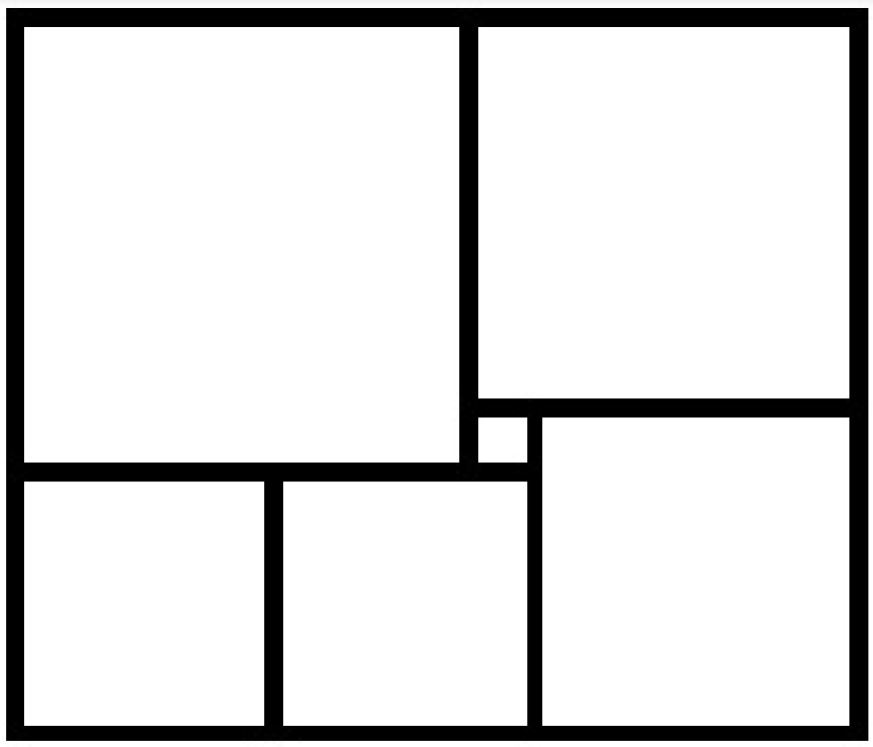
\includegraphics[width=\linewidth]{6K-46}
        \end{figure}
    \end{minipage}
\end{minipage}}
{НаписанноеРешение}
{ВерныйОтвет}{Подсказка}
\end{problem}

\begin{problem}{Решение уравнений.}{6.8.4}{6K red нужно уметь распределительный закон для скобочек}{(лёгкая)}
{Длина прямоугольного участка в $4$ раза больше ширины. Если длину увеличить на $2$ м, а ширину уменьшить на $5$ м, то площадь участка уменьшится на $190$ м$^{2}$. Каковы размеры данного участка?}
{Мы не знаем длину и ширину участка. Пусть длина участка равна $l$ метров, а ширина равна $s$ метров. Тогда, во-первых, $l = 4s$. А во-вторых, так как площадь уменьшилась на 190 квадратных метров, $(l + 2)(s - 5) = ls - 190$. Учитывая, что $l = 4s$: $(4s + 2)(s - 5) = 4s^2 - 190$. Раскрываем скобки по распределительному закону: $4s^2 - 20s + 2s - 10 = 4s^2 - 190$. Данное выражение можно упростить: приводим подобные члены, $4s^2$ сокращаются: $-18s - 10 = -190$.\\
Прибавляем 10 к обеим частям уравнения, а затем делим на $-18$: $-18s = -180 \;\Rightarrow\; s = (-180) : (-18) = 10$. Итого, ширина участка была равна 10 метрам, а значит, длина была равна 40 метрам (так как она в четыре раза больше).\smallskip\\ Сделаем проверку, что мы всё решили верно:\\
После преобразований длина составляет 42 метра, а ширина~--- 5 метров. Поэтому площадь в этом случае будет равна $42 \cdot 5 = 210$ м$^{2}$, площадь нашего участка без каких-либо изменений составляет $40 \cdot 10 = 400$ м$^{2}$. Разница площадей равна $400 - 210 = 190$ м$^{2}$, что и требовалось по условию.}
{Размеры данного участка~--- $10 \times 40$ метров.}{Обозначь неизвестные длину и ширину двумя переменными, и составь два уравнения. После приведения подобных членов уравнения упроcтятся.}
\end{problem}

\begin{problem}{Решение уравнений.}{6.8.4}{6K \textcolor{red}{\textbf{$\spadesuit$}} многопунктовая}{*}
{Решить уравнения: \\a) $\;\displaystyle \frac{3}{4} : 1\frac{1}{14} = 1{,}2 : (25 - 0{,}4x)$; \hfill b) $\;\displaystyle 1\frac{17}{35} : 2\frac{3}{5} = \left(9{,}95 - \frac{3{,}6}{x}\right) : 5$.}
{а) $\;\displaystyle \frac{3}{4} : 1\frac{1}{14} = 1{,}2 : \left(25 - \frac{10}{7}x\right) \;\Rightarrow \;\displaystyle \frac{3}{4} : \frac{15}{14} = 1{,}2 : \left(25 - \frac{10}{7}x\right)\;\Rightarrow \;$\\ $ \displaystyle \frac{3}{4} \cdot \frac{14}{15} = 1{,}2 : \left(25 - \frac{10}{7}x\right) \;\Rightarrow \;\displaystyle \frac{7}{10} = 1{,}2 : \left(25 - \frac{10}{7}x\right)$ \\ Умножим обе части уравнения на $\displaystyle\left(25 - \frac{10}{7}x\right)$: $\;\;\displaystyle \frac{7}{10} \cdot \left(25 - \frac{10}{7}x\right) = 1{,}2 $ \smallskip\\ Раскроем скобки:  $\displaystyle\frac{7}{10}\cdot 25 - \frac{7}{10} \cdot \frac{10}{7}x = 1{,}2 \;\;\Rightarrow \;\;\displaystyle \frac{35}{2} - x = 1{,}2$. <<Перенесём>> иксы вправо, а числа влево (то есть, прибавим к обеим частям уравнения $x - 1{,}2$) $\;\Rightarrow \; \displaystyle x = \frac{35}{2} - 1{,}2 = 17{,}5 - 1{,}2 = 16{,}3$. Уравнение решено.
\bigskip\\
b) $\;\displaystyle 1\frac{17}{35} : 2\frac{3}{5} = \left(9{,}95 - \frac{3{,}6}{x}\right) \!:\!5 \;\Rightarrow\; \frac{52}{35} : \frac{13}{5} = \left(9{,}95 - \frac{3{,}6}{x}\right)\!:\!5 \;\Rightarrow\;\\ \frac{52}{35} \cdot \frac{5}{13} = \left(9{,}95 - \frac{3{,}6}{x}\right)\!:\!5 \;\Rightarrow\; \frac{4}{7} = \left(9{,}95 - \frac{3{,}6}{x}\right) : 5$.\\ Домножим обе части уравнения на 5: $\;\displaystyle \frac{4}{7} \cdot 5 = 9{,}95 - \frac{3{,}6}{x} \;\Rightarrow\; \frac{20}{7} = 9{,}95 - \frac{3{,}6}{x}$. \\ Вычтем $9{,}95$ из обеих частей, получим что $\;\displaystyle\frac{20}{7} - 9{,}95 = -\frac{3{,}6}{x}$.\\ Приводим дроби к общему знаменателю и вычитаем: \smallskip\\$ \; \displaystyle\frac{20}{7} - \frac{199}{20} = \frac{20\cdot20 - 7\cdot199}{140} = -\frac{993}{140} = -\frac{3{,}6}{x}$.\\
Домножим обе части уравнения на $-1$, а затем решим пропорцию: $\displaystyle\frac{993}{140} = \frac{3{,}6}{x} \;\Rightarrow\; 993x = 3{,}6\cdot140 \;\Rightarrow\; x = \frac{3{,}6 \cdot 140}{993} = \frac{36 \cdot 14}{993} = \frac{168}{331}$.}
{Решением уравнения является $\displaystyle x = 16{,}3$.\medskip\\
Решением уравнения является $\displaystyle x = \frac{168}{331}$.}{Подсказка}
\end{problem}

\begin{problem}{Решение уравнений.}{6.8.4}{6K}{(лёгкая)}
{Можно ли разлить $50$ л бензина по трём бакам так, чтобы в первом баке было на $10$ л больше, чем во втором, а во втором на $21$ литр больше, чем в третьем?}
{Пусть во второй бак залили всего $l$ литров бензина.\\ Тогда в первом баке~--- $l + 10$ литров бензина, а в третьем~--- $l - 21$ литр.\smallskip\\
Поскольку мы знаем, что всего по трём бакам было разлито 50 литров, это означает, что $(l + 10) + l + (l - 21) = 50$. Следовательно, $3l - 11 = 50 \;\Rightarrow\; 3l = 61$.\\
Получается, что $l = \frac{61}{3} = 20\frac13$ литра.\\ Выясним, сколько бензина в других баках: в первом баке будет $20\frac13 + 10 = 30\frac13$ литров бензина, а в третьем~--- $20\frac13 - 21 = -\frac23$ литра бензина.\\ Но бензина не может быть отрицательное количество!\\ Значит, разлить бензин согласно условиям задачи нам не удастся.}
{Нет, так разлить бензин по трём бакам не получится.}{Пусть в третьем баке всего $l$ литров бензина.\\ Сколько тогда будет бензина в каждом баке?}
\end{problem}

\begin{problem}{Решение уравнений.}{6.8.4}{6K}{(лёгкая)}
{Реши уравнение $\;((0{,}001 \cdot x + 2) : 0{,}3) \cdot 0{,}01 - 11{,}2 = 22{,}2$.}
{Прибавим к обеим частям уравнения $11{,}2$: уравнение останется верным:
$((0{,}001 \cdot x + 2) : 0{,}3) \cdot 0{,}01 = 33{,}4$. Теперь разделим обе части уравнения на $0{,}01$: $((0{,}001 \cdot x + 2) : 0{,}3) \cdot 0{,}01 : 0{,}01 = 33{,}4 : 0{,}01 \;\Rightarrow\; (0{,}001 \cdot x + 2) : 0{,}3 = 3340$.\\
Умножаем обе части уравнения на $0{,}3$, получаем, что $0{,}001 \cdot x + 2 = 3340 \cdot 0{,}3 \,\Rightarrow$ \\
$0{,}001 \cdot x + 2 = 1002$. Вычитаем 2: $\;0{,}001 \cdot x = 1000$. Осталось поделить на $0{,}001$, а так как это то же, что и умножение на 1000, получаем $x = 1000000$.}
{$x = 1000000$ (ровно миллион).}{Используй по очереди все 4 метода решения уравнений.}
\end{problem}

\begin{problem}{Решение уравнений.}{6.8.4}{6K}{(лёгкая)}
{Реши уравнение $\,2 \cdot (0{,}2 - 0{,}02 : (0{,}002 + 0{,}0002x)) = 0{,}3$.}
{НаписанноеРешение}
{ВерныйОтвет}{Подсказка}
\end{problem}

\begin{problem}{Решение уравнений.}{6.8.4}{6K}{*}
{Вася Пупкин прочитал книгу за $3$ дня. В первый день он прочитал $0{,}2$ всей книги и ещё $16$ страниц, во второй день~--- $0{,}3$ остатка и ещё $20$ страниц.\\ В последний день он прочитал $0{,}75$ нового остатка и последние $30$ страниц.\\ Сколько страниц было в этой книге?}
{Пусть $x$ --- количество страниц, прочитанное за последний день. Мы знаем, что это все страницы, которые оставалось прочитать, то есть $x = 0{,}75x + 30$. Следовательно, $\frac14 x = 30$, а значит $x = 120$. За день до этого было прочитано ещё 20 страниц, итого после прочтения $0{,}3$ остатка второго дня всего осталось $120 + 20 = 140$ страниц. Значит, 140 страниц составляет $0{,}7$ от того, что было на начало второго дня. Следовательно, в начале второго дня оставалось прочитать $140 : 0{,}7 = 140 \cdot\frac{10}{7} = 200$ страниц. Таким образом, всего было прочитано $0{,}2$ книги и 216 страниц. Это означает, что $216$ страниц --- $0{,}8$ страниц книги.\\ Поэтому всего в книге $216 : 0{,}8 = 216 \cdot \frac{10}{8} = 270$ страниц.}
{В этой книге было 270 страниц.}{Сколько страниц было прочитано в последний день?}
\end{problem}

\begin{problem}{Решение уравнений.}{6.8.4}{6K}{(лёгкая)}
{Чтобы наполнить ванну вместимостью $166$ л за $22$ минуты, сначала открыли кран с горячей водой, через который за $1$ минуту вливается $6{,}75$ литра. Затем этот кран закрыли и открыли кран с холодной водой, через который за $1$ минуту вливается $8{,}5$ литра. Сколько времени был открыт каждый кран?}
{НаписанноеРешение}
{ВерныйОтвет}{Подсказка}
\end{problem}

\begin{problem}{Решение уравнений.}{6.8.4}{6K}{(лёгкая)}
{Ширина прямоугольника в $3{,}2$ раза меньше длины, а периметр равен $105$ м. Найти периметр и площадь квадрата со стороной, равной ширине этого прямоугольника.

}
{Для начала найдём стороны этого прямоугольника. Пусть его ширина составляет $l$ метров. Тогда длина равна $3{,}2l$. Следовательно, его периметр равен $P = 2\cdot(l + 3{,}2l) = 2\cdot4{,}2l = 8{,}4l$. Получаем уравнение: $8{,}4l = 105$.\\ Разделим обе части уравнения на $8{,}4$: $\:l = 105 : 8{,}4 = 1050 : 84 = 50 : 4 = 12{,}5$.\\ Таким образом, ширину квадрата мы нашли --- она равна $12{,}5$ метров. Периметр квадрата с такой стороной равен $4\cdot12{,}5 = 48 + 2 = 50$ метров. Площадь этого квадрата равна $12{,}5\cdot12{,}5 = (12 + \frac12)\cdot(12 + \frac12) = 12\cdot12 + 12\cdot\frac12 + \frac12\cdot12 + \frac12\cdot\frac12 = 144 + 6 + 6 + 0{,}25 = 156{,}25$ м$^2$.}
{Периметр этого квадрата равен 50 м, площадь --- $156{,}25$ м$^2$.}{Пусть ширина прямоугольника равна $l$. Чему тогда равна длина? Периметр? Найди $l$ и вычисли периметр и площадь требуемого квадрата.}
\end{problem}

\begin{problem}{Решение уравнений.}{6.8.4}{6K}{(лёгкая)}
{Два робота, робот Анатолий и робот Василий, чистят картошку. Один из них очищал в минуту две картофелины, а второй~--- три картофелины. Вместе они очистили $400$ штук. Сколько времени проработал каждый, если второй робот работал на $25$ минут больше первого?}
{Для решения задачи допустим, что первый робот работал $T$ минут. Тогда второй работал $T + 25$ минут. Поскольку первый робот чистит 2 картофелины в минуту, а второй~--- 3, получаем, что первый робот очистит $2T$ картофелин. Второй робот за всё время очистит $3 \cdot (T + 25) = 3T + 75$ картофелин. Поскольку всего успешно очищенных картофелин 400, $400 = 2T + 3T + 75 = 5T + 75$. Вычтем 75 картофелин из обеих частей уравнения: $325 = 5T$. Уменьшим количество картошки в 5 раз и слева, и справа: $65 = T$. Значит, первый робот работал $65$ минут. Как мы знаем, второй робот работал на 25 минут больше, а значит, он работал всего $65 + 25 = 90$ минут.}
{Первый робот работал 65 минут, второй~--- 90 минут.}{Пусть первый робот работал $T$ минут. Сколько картофелин он успеет очистить? Сколько времени будет работать второй робот?}
\end{problem}

\begin{problem}{Решение уравнений.}{6.8.4}{6K}{*}
{Если бы Иван Никифорович отдал Ивану Ивановичу половину своих гусей, то у Ивана Ивановича стало бы на десять гусей больше, чем у Ивана Никифоровича. Сколько гусей было у Ивана Ивановича?}
{Допустим, что всего у Ивана Никофоровича было $x$ гусей, а у Ивана Ивановича было $y$ гусей. Тогда Иван Никифорович отдаёт $\frac x2$ гусей. Значит, у Ивана Никифоровича останется $\frac x2$ гусей, а у Ивана Ивановича будет $y + \frac x2$ гусей. В таком случае у Ивана Ивановича будет больше гусей, чем у Ивана Никифоровича: а именно, на $(y + \frac x2) - \frac x2 = y$ гусей больше. Следовательно, $y = 10$.\\ То есть вначале у Ивана Ивановича было 10 гусей.}
{Вначале у Ивана Ивановича было 10 гусей.\\
\textbf{Комментарий:} Отмечу, что в рамках данной задачи, узнать сколько всего гусей было у Ивана Никифоровича не представляется возможным.}{Пусть у Ивана Никифоровича сначала было всего $x$ гусей, а у Ивана Ивановича было $y$ гусей. Сколько гусей станет у каждого из них после обмена?}
\end{problem}

\begin{problem}{Решение уравнений.}{6.8.4}{6K}{(лёгкая)}
{В классе число отсутствующих учеников составляет $1/8$ числа присутствующих. Если из класса выйдут ещё два ученика, то будет отсутствовать $20\%$ числа учеников, оставшихся в классе. Сколько всего в классе учеников?}
{НаписанноеРешение}
{ВерныйОтвет}{Подсказка}
\end{problem}

\begin{problem}{Решение уравнений.}{6.8.4}{6K}{(лёгкая)}
{Длина одного прямоугольника равна $32$ см, а другого~--- $15$ см.\\ Ширина второго прямоугольника на $6$ см больше ширины первого.\\ Найди их площади, если известно, что площадь первого прямоугольника на \\$46$ см$^{2}$ больше площади второго прямоугольника.}
{Пусть ширина первого прямоугольника равна $b$ см. Тогда, раз ширина второго на 6 см больше, она равна $b + 6$ см. Каковы площади первого и второго прямоугольников? Первый прямоугольник имеет длину 32 см и ширину $b$ см, значит его площадь равна $32b$ см$^2$. Второй прямоугольник имеет длину 15 см и ширину $b + 6$ см, поэтому его площадь --- $15(b + 6) = 15b + 90$ см$^2$. Раз площадь первого на 46 см$^2$ больше, получаем уравнение: $32b = 15b + 90 + 46 = 15b + 136$. Вычтем $15b$ из обеих частей уравнения: получаем, что $32b - 15b = 136$, то есть $17b = 136$. Делим обе части на 17: $b = 136 : 17 = 8$. Итого, $b = 8$.\\
Находим площади: площадь первого прямоугольника равна $32\cdot8 = 256$ см$^2$, а площадь второго равна $15\cdot(8 + 6) = 15\cdot14 = 210$ см$^2$. Всё совпадает.}
{Площади этих прямоугольников --- 256 и 210  см$^2$.}{Обозначь ширину первого прямоугольника за $b$ и составь уравнение, выразив через $b$ площади первого и второго прямоугольников.}
\end{problem}

\begin{problem}{Решение уравнений.}{6.8.4}{6K}{(лёгкая)}
{Найти решение уравнения $\displaystyle 1\frac{3}{25} : 0{,}8 = 0{,}7 \cdot (11{,}9 - \chi)$.}
{НаписанноеРешение}
{ВерныйОтвет}{Подсказка}
\end{problem}

\begin{problem}{Решение уравнений.}{6.8.4}{6K}{(лёгкая)}
{Найти решение уравнения $\displaystyle 2\frac{2}{25} : 0{,}08 = 1{,}3 \cdot (22{,}2 - \chi)$.}
{НаписанноеРешение}
{ВерныйОтвет}{Подсказка}
\end{problem}

\begin{problem}{Решение уравнений.}{6.8.4}{6K}{(лёгкая)}
{Найти решение уравнения $\;\displaystyle \frac{7}{8} - 2{,}5 : \left(32{,}8 + 3|y|\right) = 0{,}8125$.}
{НаписанноеРешение}
{ВерныйОтвет}{Подсказка}
\end{problem}

\begin{problem}{Решение уравнений.}{6.8.4}{6K}{(лёгкая)}
{Запас мака распределили между тремя пекарнями. Количество мака во второй пекарне составляет $60\%$ от количества мака в первой пекарне, а количество мака в третьей пекарне составляет $150\%$ от количества мака во второй пекарне.\\ Сколько мака в каждой пекарне, если всего во всех пекарнях его $3$ тонны?}
{НаписанноеРешение}
{ВерныйОтвет}{Подсказка}
\end{problem}

\begin{problem}{Решение уравнений.}{6.8.4}{6K}{(лёгкая)}
{Найти решение уравнения $\displaystyle15\frac{3}{35} : 8{,}8 = \frac{5}{7} \cdot (9{,}7 - |x|)$.}
{НаписанноеРешение}
{ВерныйОтвет}{Подсказка}
\end{problem}

\begin{problem}{Решение уравнений.}{6.8.4}{6K}{(лёгкая)}
{Найти решение уравнения $\displaystyle\left((3{,}33 - p) : 1{,}5 + 17{,}4 : 29\right) : (25 \cdot 0{,}16) - 0{,}017 = 0{,}388$.

}
{НаписанноеРешение}
{ВерныйОтвет}{Подсказка}
\end{problem}

\begin{problem}{Решение уравнений.}{6.8.4}{6K}{(лёгкая)}
{Найти решение уравнения $\;\displaystyle x - \left(\frac{4}{15}x + \frac{4}{9}\left(x - \frac{4}{15}x\right)\right) = \frac{4}{15}x + \frac{4}{9}\left(x - \frac{4}{15}x\right) - 25$.

}
{НаписанноеРешение}
{ВерныйОтвет}{Подсказка}
\end{problem}

\begin{problem}{Решение уравнений.}{6.8.4}{6K}{(лёгкая)}
{Решить уравнение $\displaystyle\left(x - \frac{1}{8}\right) + 4 \cdot \frac{1}{7} = 5{,}1$.}
{НаписанноеРешение}
{ВерныйОтвет}{Подсказка}
\end{problem}

\begin{problem}{Решение уравнений.}{6.8.4}{6K}{(лёгкая)}
{\vspace{-7mm}\\\begin{minipage}{\linewidth}
    \begin{minipage}{0.65\linewidth}
    \vspace{4mm}
    На рисунке справа прямоугольник $ABCD$ разделён на четыре маленьких прямоугольника, да так, что периметры всех этих прямоугольников одинаковы.\smallskip\\ Известно, что $AB = 18$ см, $BC = 16$ см.\\ Найти стороны прямоугольников.

    \end{minipage}
    \hspace{0.04\linewidth}
    \begin{minipage}{0.29\linewidth}
        \begin{figure}[H]
        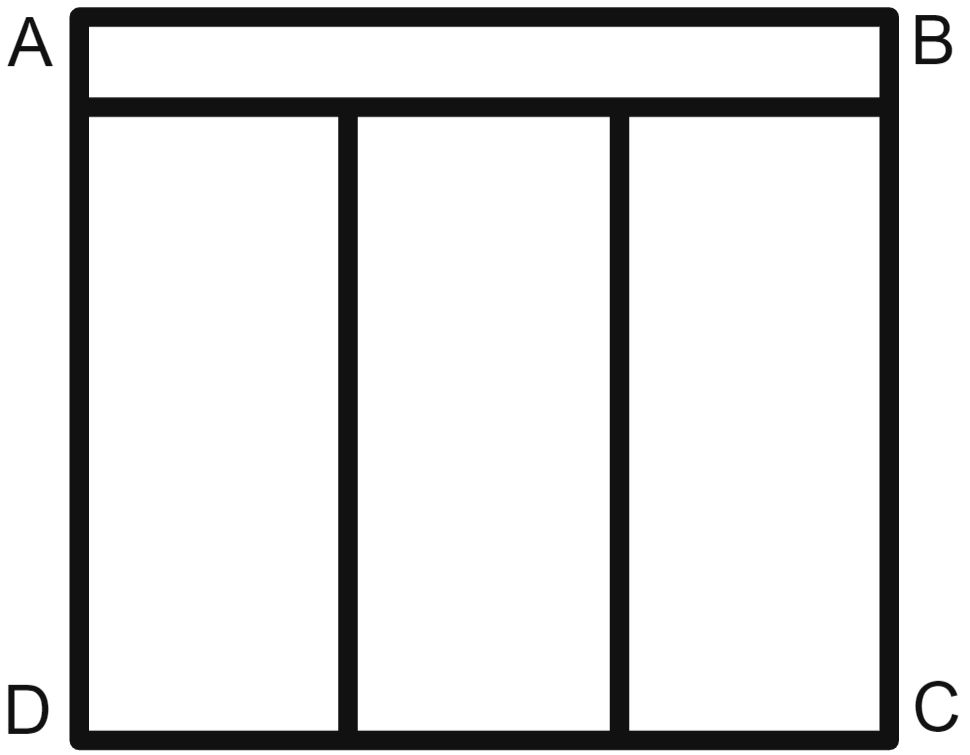
\includegraphics[width=\linewidth]{6K-34}
        \end{figure}
    \end{minipage}
\end{minipage}}
{Для решения задачи нужно найти длины всех отрезочков, которые составляют указанные прямоугольники. Отметим, что так как все три нижних прямоугольника имеют одну и ту же высоту, то поскольку периметры всех прямоугольников равны, то и ширина у всех этих прямоугольников одинаковая, то есть $CD$ делится на три равные части. $CD = AB = 18$ см, поэтому ширина каждого из нижних прямоугольников равна $18 : 3 = 6$ см. Нам неизвестна ширина верхнего прямоугольника. Допустим, что она равна $L$ см. Тогда, так как $BC = 16$ см, высота нижних трёх прямоугольников равна $16 - L$ см. Значит, периметр верхнего прямоугольника равен $P_{\text{верх}} = 2\cdot(18 + L) = 36 + 2L$ см, а периметр нижнего прямоугольника равен $P_{\text{нижн}} = 2\cdot(6 + 16 - L) = 44 - 2L$ см. Периметры этих двух прямоугольников равны, а значит $36 + 2L = 44 - 2L$, откуда $2L + 2L = 44 - 36 \;\Rightarrow\; 4L = 8 \;\Rightarrow\; L = 2$ см.\\ Таким образом, стороны верхнего прямоугольника равны 2 и 18 сантиметров, а стороны каждого из нижних трёх прямоугольников равны 6 и 14 сантиметров.}
{Стороны прямоугольников равны 2 и 18 сантиметров для верхнего и 6 и 14 сантиметров для каждого из нижних прямоугольников, соответственно.}{Чему равна ширина нижних прямоугольников?\\ Пусть $L$~--- ширина верхнего прямоугольника.}
\end{problem}

\begin{problem}{Решение уравнений.}{6.8.4}{6K}{(лёгкая)}
{$a + b = 8481$. Одно из чисел оканчивается на $0$.\\ Если его вычеркнуть, получится второе число. Что это за числа?}
{Поскольку меньшее число получается из большего вычёркиванием нуля, это значит, что большее число в 10 раз больше. Пусть меньшее число --- это $b$. Тогда наши числа --- $b$ и $10b$. Значит, сумма чисел $a + b = 11b$. То есть, $11b = 8481$. Поделив обе части этого уравнения на 11, получаем $b = 8481 : 11 = 771$.\\ Большее число получается из меньшего приписыванием нуля: $a = 7710$.\smallskip\\
Проверка: $a + b = 7710 + 771 = 8481$.}
{Это числа 771 и 7710.}{Во сколько раз отличаются числа, если одно получается из другого вычёркиванием нуля? Составь уравнение и реши его.}
\end{problem}

\begin{problem}{Решение уравнений.}{6.8.4}{6K}{(лёгкая)}
{Найти значение переменной $\alpha$, являющееся решением уравнения $$\displaystyle\frac{3}{7} : 1\frac{1}{14} = 0{,}4 : (4 - \alpha).$$

}
{НаписанноеРешение}
{ВерныйОтвет}{Подсказка}
\end{problem}

\begin{problem}{Решение уравнений.}{6.8.4}{6K}{(лёгкая)}
{Бабушка сказала внукам: <<Если я испеку каждому из вас по два пирожка, у меня останется теста на три лишних пирожка, а если я захочу испечь каждому из вас по три пирожка, то мне не хватит теста на два пирожка>>.\\ Сколько внуков у бабушки?}
{НаписанноеРешение}
{ВерныйОтвет}{Подсказка}
\end{problem}

\begin{problem}{Решение уравнений.}{6.8.4}{6S}{(лёгкая)}
{Дочери сейчас 3 года, а её матери~--- 31 год.\\ Через сколько лет мать будет втрое старше дочери?}
{Пусть $y$~--- количество лет, которое должно пройти до этого момента. Тогда дочь станет старше на $y$ лет, и ей будет $3 + y$ лет, а мать также станет старше на $y$ лет, и ей будет $31 + y$ лет. То есть, поскольку мать будет втрое старше дочери, $31 + y = 3 \cdot (3 + y) = 9 + 3y$. Вычитаем из обеих частей уравнения $y$ и 9: приходим к уравнению $31 - 9 = 22 = 2y$. Уменьшаем обе части уравнения вдвое: при этом уравнение остаётся верным, и мы получаем, что $y = 11$.\\
Проверка: $3 + 11 = 14$, $\,31 + 11 = 42$, $\,42 = 3 \cdot 14$.}
{Мать будет втрое старше дочери через 11 лет.}{Пусть искомое количество лет равно $y$.}
\end{problem}

\begin{problem}{Решение уравнений.}{6.8.4}{6S}{(лёгкая)}
{Деду 56 лет, а внуку 14. Когда дедушка будет вдвое старше своего внука?}
{Допустим, пройдёт $t$ лет. Тогда дедушке будет $56 + t$ лет, а внуку --- $14 + t$ лет. Если дедушка будет вдвое старше, то в этот момент $56 + t$ вдвое больше чем $14 + t$, то есть $56 + t = 2\cdot(14 + t)$. Значит, $56 + t = 28 + 2t$. Вычитаем 28 из обеих частей: получаем, что $28 + t = 2t$. Вычитаем $t$ из обеих частей: $\,28 = t$.\\ То есть, получается, что это произойдёт через 28 лет.\smallskip\\ Проверка: внуку будет $14 + 28 = 42$ года, а дедушке $56 + 28 = 84$ года.}
{Дедушка будет вдвое старше внука через 28 лет.}{Пусть до этого момента времени прошло $t$ лет.\\ Сколько теперь лет внуку? Сколько деду? Какое уравнение можно записать?}
\end{problem}

\begin{problem}{Решение уравнений.}{6.8.4}{6S}{(лёгкая)}
{Отец старше сына в 4 раза, а сумма их возрастов составляет 50 лет.\\ Через сколько лет отец станет втрое старше сына?}
{Пусть сыну $x$ лет, тогда отцу $4x$ лет. Сумма их возрастов равна $5x$. Значит, $5x = 50$. Уменьшаем обе части уравнения в 5 раз (делим на 5), получаем, что $x = 10$, то есть на данный момент сыну 10 лет, а отцу 40. Пусть $t$~--- время, которое должно пройти до того момента, когда отец окажется втрое старше.\\ Тогда в этот момент сыну будет $10 + t$ лет, а отцу~--- $40 + t$ лет. Значит, $40 + t = 3 \cdot (10 + t) = 30 + 3t$. Вычитаем из обеих частей уравнения $t$: получаем также верное уравнение $40 = 30 + 2t$. Вычитаем 30 из обеих частей уравнения: $10 = 2t$. Уменьшаем обе части уравнения вдвое и находим, что $t = 5$.\\ То есть это произойдёт через 5 лет (сыну тогда будет 15, а отцу 45).}
{Через 5 лет.}{Пусть сыну сейчас $x$ лет. Чему тогда равна сумма возрастов отца и сына? Пусть $t$~--- время до того момента, когда отец станет втрое старше сына.}
\end{problem}

\begin{problem}{Решение уравнений.}{6.8.4}{6S}{(лёгкая)}
{Дочери сейчас 7 лет, а отцу в пять раз больше.\\ Через сколько лет отец станет втрое старше дочери?}
{НаписанноеРешение}
{ВерныйОтвет}{Подсказка}
\end{problem}

\begin{problem}{Решение уравнений.}{6.8.4}{6S}{(лёгкая)}
{Отец старше сына на 24 года.\\ Сколько лет сыну, если через 3 года он будет в 5 раз моложе отца?}
{НаписанноеРешение}
{ВерныйОтвет}{Подсказка}
\end{problem}

\begin{problem}{Решение уравнений.}{6.8.4}{6S}{(лёгкая)}
{Бабушке 61 год, а внуку 17 лет.\\ Сколько лет назад бабушка была старше внука в 5 раз?}
{НаписанноеРешение}
{ВерныйОтвет}{Подсказка}
\end{problem}

\begin{problem}{Решение уравнений.}{6.8.4}{6S}{(лёгкая)}
{У 35-летнего отца 4 сына. Каждый моложе другого на 2 года, причём старшему 8 лет. Когда всем детям вместе будет столько же лет, сколько и отцу?}
{Раз старшему 8 лет, и сыновья каждый моложе друг друга на 2 года, то следующему по старшинству сыну 6 лет, следующему~--- 4, а самому младшему сыну 2 года. Значит, сейчас им вместе $2 + 4 + 6 + 8 = 20$ лет. За год каждый из сыновей станет на год старше, а значит, сумма их возрастов вырастет на 4.\\ Пусть через $t$ лет всем детям будет столько же лет, сколько и отцу.\\ Тогда $20 + 4t = 35 + t$, откуда $4t - t = 35 - 20 \;\Rightarrow\; 3t = 15 \;\Rightarrow\; t = 5$. \\
Сделаем проверку: через 5 лет отцу будет 40 лет, а возрасты сыновей будут $7$, $9$, $11$, $13$ лет. Суммарный возраст также равен 40 годам.}
{Через 5 лет детям вместе будет столько же лет, сколько и отцу.}{Как изменится суммарный возраст сыновей через один год?}
\end{problem}

\begin{problem}{Решение уравнений.}{6.8.4}{6S}{(лёгкая)}
{В конференции Zoom число отсутствующих учеников составляло $\frac{1}{6}$ часть от числа присутствующих. После того, как из конференции вышел один ученик, число отсутствующих стало равно $\frac{1}{5}$ числа присутствующих.\\ Сколько учеников участвовало в конференции?}
{Как и всегда, в этой задаче есть неизвестная нам величина~--- сколько учеников присутствовало в конференции в начале. Обозначим это число за $x$. Тогда отсутствовало $\frac16 x$. Посмотрим, что произошло, когда один ученик покинул конференцию. Теперь присутствует $x - 1$ ученик, а отсутствует $\frac16 x + 1$ учеников.\\ Но мы знаем ещё кое-что! Нам известно, что теперь число отсутствующих составляет $\frac15$ числа присутствующих, то есть $\frac16 x + 1 = \frac15 (x - 1)$. Уравнение составлено, можно приступать к решению. Для начала раскроем скобки: $\,\frac16 x + 1 = \frac15 x - \frac15$.\\ Переносим иксы влево, а числа вправо (вычитаем из обеих частей уравнения $1 + \frac15 x$): $\:\frac16 x + 1 = \frac15 x - \frac15 \;\Rightarrow\; \,\frac16 x + 1 - (1 + \frac15 x) = \frac15 x - \frac15 - (1 + \frac15 x) \;\Rightarrow$\smallskip\\ $\Rightarrow\; \frac16 x - \frac15 x = -\frac15 - 1$. Приводим дроби к общему знаменателю, получаем, что\\
$\frac{5}{30} x - \frac{6}{30} x = -\frac65 \;\Rightarrow\; -\frac{1}{30} x = -\frac{6}{5} \;\Rightarrow\; x = \left(-\frac{6}{5}\right) : \left(-\frac{1}{30}\right) = \left(-\frac{6}{5}\right) \cdot (-30) = 36$.\smallskip\\
Итого, в конференции участвовало 36 учеников.}
{В конференции участвовало 36 учеников.}{Пусть $x$~--- число учеников, участвовавших в конференции.}
\end{problem}

\begin{problem}{Решение уравнений.}{6.8.4}{6S}{(лёгкая)}
{Грузовик проезжает некоторое расстояние за $10$ ч. Если бы он проезжал в час на $10$ км больше, то ему потребовалось бы на тот же путь $8$ часов.\\ Каким было расстояние и скорость движения грузовика?}
{Пусть $v$ км/ч~--- скорость движения грузовика. Если бы его скорость была на 10 км/ч больше, то она была бы равна $v + 10$ км/ч. Поскольку путь тот же, это означает, что $10 \cdot v = 8 \cdot (v + 10) \;\Rightarrow\; 10v = 8v + 80$.\\ Вычитаем $8v$ из обеих частей уравнения, получаем, что $2v = 80$, откуда, после деления обеих частей уравнения на 2, $v = 40$. Значит, грузовик за час проезжает 40 километров, а общее расстояние равно $40 \cdot 10 = 400$ километров.\\ Проверка: если бы скорость была 50 км/ч, то тогда $400 = 50 \cdot 8$.}
{Скорость грузовика~--- 40 км/ч, расстояние составляет 400 километров.}{Пусть скорость грузовика равна $v$.}
\end{problem}

\begin{problem}{Решение уравнений.}{6.8.4}{6S}{(лёгкая)}
{Кроликов было на 7 больше, чем фазанов, а ног все кролики имели на 48 больше, чем все фазаны. Сколько было кроликов и сколько~--- фазанов?}
{НаписанноеРешение}
{ВерныйОтвет}{Подсказка}
\end{problem}

\begin{problem}{Решение уравнений.}{6.8.4}{6S}{(лёгкая)}
{Если учитель посадит учеников своего класса на скамейки по трое, то восьмерым ученикам не хватит места. Если же он посадит на каждую скамейку по шесть учеников, то останется 16 свободных мест. Сколько учеников в классе?}
{Первым делом при решении задачи нужно ввести неизвестные.\\ Пусть $x$~--- число учеников в классе, а $n$~--- количество скамеек. Тогда получаем следующие уравнения: $x = 3n + 8$ и $6n = x + 16$ (так как можно усадить и всех учеников, и ещё 16 человек). Но тогда $6n = (3n + 8) + 16 \;\Rightarrow\; 6n = 3n + 24 \;\Rightarrow\; 3n = 24 \;\Rightarrow\; n = 8$, то есть скамеек всего 8. Теперь можно найти и количество учеников: $x = 3n + 8 = 3\cdot8 + 8 = 24 + 8 = 32$. Итого, в классе всего 32 ученика.}
{В классе было 32 ученика.}{Пусть $x$~--- количество учеников в классе, а $n$~--- число скамеек.\\ Какие уравнения тогда получаются?}
\end{problem}

\begin{problem}{Решение уравнений.}{6.8.4}{6S}{(лёгкая)}
{Стая галок опустилась на деревья по 35 на каждое. Остались без места 4 галки. Когда галки сели по 38 на каждое дерево, то осталось 32 свободных места.\\ Сколько было галок и сколько деревьев?}
{Пусть всего было $T$ деревьев и $B$ галок. Тогда в первом случае всего на деревьях сидит $35T$ галок, а всего галок $B = 35T + 4$. Во втором случае $B = 38T - 32$. Следовательно, $35T + 4 = 38T - 32$. Прибавляем 32 к обеим частям уравнения и вычитаем $35T$: получаем, что $36 = 3T$. Делим на 3: $\,12 = T$.\\ Так мы нашли число деревьев. Галок же всего было $B = 35\cdot12 + 4 = 424$.}
{Всего было 12 деревьев и 424 галки.}{Пусть всего было $T$ деревьев и $B$ галок. Какие уравнения получатся?}
\end{problem}

\begin{problem}{Решение уравнений.}{6.8.4}{6S}{(лёгкая)}
{Прилетели галки, сели на палки. Сели по одной~--- галка лишняя.\\ Сели по две~--- палка лишняя. Сколько было галок? А сколько было палок?}
{Допустим, что галок было $g$, а палок было $p$. Тогда, когда галки садились на палки по одной, одна галка оказалась лишней, а значит, $g = p + 1$.\\ С другой стороны, когда галки садились по две, одна палка оказалась свободной, а значит всего сидит $2(p - 1) = g$ галок. Несложно догадаться, что тогда $2(p - 1) = g = p + 1$. Получилось обычное уравнение $2(p - 1) = p + 1$. Раскроем скобки: $\;2p - 2 = p + 1$. Прибавим к обеим частям уравнения 2: $\;2p = p + 3$.\\
Вычтем из обеих частей уравнения $p$: $\;p = 3$. Значит, всего было 3 палки. А сколько было галок? Мы знаем, что $g = p + 1 = 3 + 1 = 4$. То есть галок было 4.\\
Проверка: $4 = 3 + 1$ (сели по одной, одной места не хватило) и $4 = 2\cdot(3 - 1)$ (сели по две, одна палка из трёх пустует).}
{Галок было 4, а палок было 3.}{Пусть галок было $g$, а палок было $p$. Нужно составить два уравнения.}
\end{problem}

\begin{problem}{Решение уравнений.}{6.8.4}{56}{(лёгкая)}
{У Лёши было $12$ больших мелков, некоторые из них он разломал на $3$ части, и в итоге у него стало $24$ мелка. Сколько больших мелков у него осталось?}
{НаписанноеРешение}
{ВерныйОтвет}{Подсказка}
\end{problem}

\begin{problem}{Решение уравнений.}{6.8.4}{7A}{(лёгкая)}
{Поезд, двигаясь равномерно со скоростью 57 км/ч, проезжает мимо идущего в том же направлении параллельно путям со скоростью 5 км/ч пешехода за 45 секунд. Найти длину поезда в метрах.}
{НаписанноеРешение}
{ВерныйОтвет}{Подсказка}
\end{problem}

\begin{problem}{Решение уравнений.}{6.8.4}{56}{(лёгкая)}
{Периметр первого прямоугольника на $6$ см больше периметра второго, а ширина первого прямоугольника на $4$ см меньше длины второго. На сколько сантиметров длина первого прямоугольника больше ширины второго прямоугольника?}
{Как известно, периметр прямоугольника со сторонами $a$ и $b$ равен $P = 2a + 2b$. Поэтому, если $\text{Ш}_1$ и $\text{Д}_1$ --- ширина и длина первого прямоугольника, а $\text{Ш}_2$ и $\text{Д}_2$ --- ширина и длина второго прямоугольника, то согласно первому условию $2\text{Ш}_1 + 2\text{Д}_1 = 2\text{Ш}_2 + 2\text{Д}_2 + 6$, откуда $\text{Ш}_1 + \text{Д}_1 = \text{Ш}_2 + \text{Д}_2 + 3$ (деление обеих частей уравнения на 2). Также мы знаем, что $\text{Ш}_1 = \text{Д}_2 - 4$. После некоторых размышлений становится понятно, что можно в уравнении выше заменить $\text{Ш}_1$ на $\text{Д}_2 - 4$, раз это одно и то же. Значит, $\text{Д}_2 - 4 + \text{Д}_1 = \text{Ш}_2 + \text{Д}_2 + 3$. Вычитаем $\text{Д}_2$ из обеих частей уравнения: $\text{Д}_1 - 4 = \text{Ш}_2 + 3$. Прибавим 4 к обеим частям уравнения: $\text{Д}_1 = \text{Ш}_2 + 7$. Оказывается, это ответ на задачу! Ведь написанное означает, что длина первого прямоугольника на 7 сантиметров больше, чем ширина второго.}
{Длина первого прямоугольника на 7 см больше, чем ширина второго.}{Обозначь ширину и длину первого и второго прямоугольников и составь два уравнения.}
\end{problem}

\begin{problem}{Решение уравнений.}{6.8.4}{56}{(лёгкая)}
{Решить уравнение: $\;350{,}02 : (7{,}05 \cdot x - 20{,}29) - 306{,}45 = 100{,}55$.}
{НаписанноеРешение}
{ВерныйОтвет}{Подсказка}
\end{problem}

\begin{problem}{Решение уравнений.}{6.8.4}{56}{(лёгкая)}
{В первый день со склада вывезли $\frac{3}{5}$ всей муки, во второй~--- 30\% оставшейся, а в третий~--- остальные $325$ центнеров. Сколько центнеров муки было на складе?}
{НаписанноеРешение}
{ВерныйОтвет}{Подсказка}
\end{problem}

\begin{problem}{Решение уравнений.}{6.8.4}{6K red это не уравнения, а начало квадратных - составление выражений МБ}{(лёгкая)}
{У Василия Ивановича был квадратный участок земли, однако после того, как одну сторону участка уменьшили на $3$ метра, а другую сторону увеличили на $3$ метра, площадь участка составила $432$ м$^{2}$.\\ Какие размеры были у участка в начале?}
{Как и всегда при решении задач, введём неизвестную~--- обозначим за $a$ сторону этого квадратного участка в начале.\\

\begin{minipage}{\linewidth}
    \begin{minipage}{0.5\linewidth}
    Посмотрим, как выглядит участок после увеличений и уменьшений сторон: см. рисунок справа.\\ Теперь это уже не квадрат, а прямоугольник~--- одна его сторона равна $a + 3$, а другая равна $a - 3$.\\
    Значит, по формуле для площади прямоугольника из условия задачи (площадь прямоугольника после этих операций нам известна) получаем уравнение: $$(a + 3)\cdot(a - 3) = 432.$$
    \end{minipage}
    \hspace{0.05\linewidth}
    \begin{minipage}{0.44\linewidth}
        \begin{figure}[H]
        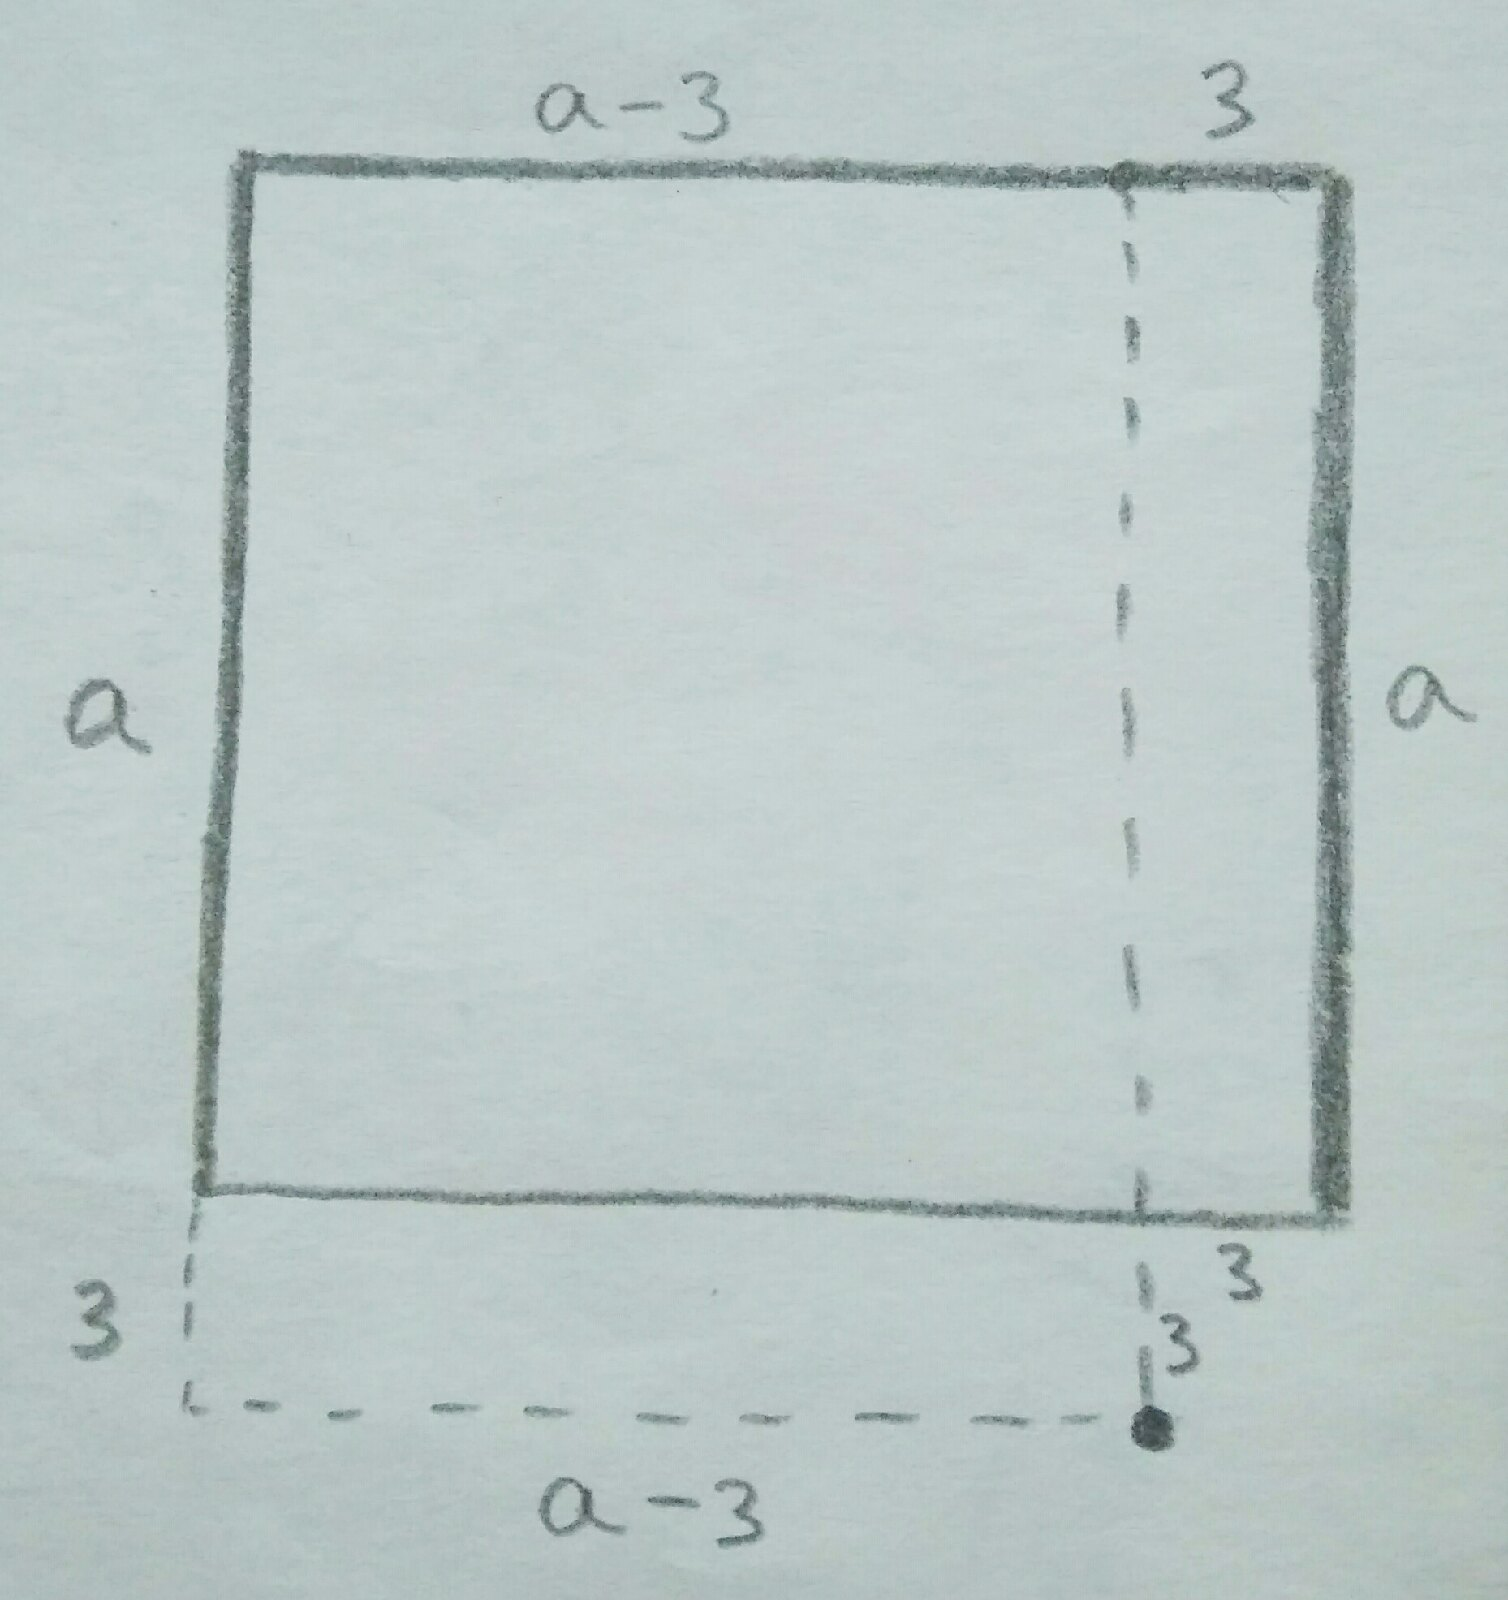
\includegraphics[width=\linewidth]{sol1.jpg}
        \end{figure}
    \end{minipage}
\end{minipage}
Можно уже начинать подбирать ответ (произведение двух чисел даёт 432), а можно ещё упростить: cогласно распределительному закону, $(a + 3)\cdot(a - 3) = a(a - 3) + 3(a - 3) = a\cdot a - 3a + 3a - 9 = a^2 - 9$.\smallskip\\ Поэтому приходим к уравнению $a^2 - 9 = 432 \Rightarrow a^2 = 441$.
Такое уравнение мы пока что умеем решать только подбором: если $a = 20$, то $a\cdot a = 400 \Rightarrow$ $a$ должно быть больше 20... Берём 21: $\;21\times21 = 21 + 420 = 441$. Победа.}
{В начале у участка были размеры $21\times 21$ метр.}{Подсказка}
\end{problem}

\begin{problem}{Решение уравнений.}{6.8.4}{6K red свойства корня/степени}{(лёгкая)}
{Решить уравнение: $\;\displaystyle x^{2} = \frac{28}{3} \cdot \frac{8}{35} \cdot \frac{3}{10}$.}
{НаписанноеРешение}
{ВерныйОтвет}{Подсказка}
\end{problem}

\begin{problem}{Решение уравнений.}{6.8.4}{6S}{(лёгкая)}
{Расстояние между двумя городами турист проехал за два дня.\\ В первый день он проехал половину пути и ещё 24 км. Во второй день ему осталось проехать расстояние в три раза меньшее, чем в первый день.\\ Найти расстояние между городами.}
{Пусть общее расстояние между городами равно $L$. Тогда, поскольку за второй день осталось проехать расстояние, в три раза меньшее, чем в первый день, это означает, что в первый день было пройдено $\frac34 L$, а во второй --- $\frac14 L$.\smallskip\\ Но так как в первый день турист проехал половину пути и ещё 24 км, это означает, что $\frac12 L + 24 = \frac34 L$. Вычитаем из обеих частей полученного уравнения $\frac12 L$: получаем, что $24 = \frac34 L - \frac12L \;\Rightarrow\; 24 = \frac14 L$. Теперь умножим обе части уравнения на 4: $\;96 = L$.\\
Итого, расстояние между городами составляет 96 километров.}
{Расстояние между этими городами --- 96 километров.}{Пусть расстояние между городами равно $L$.\\ Какую часть $L$ осталось проехать туристу во второй день?}
\end{problem}

\begin{problem}{Решение уравнений.}{6.8.4}{6S}{(лёгкая)}
{Торговка, сидя на рынке, размышляла: <<Если бы к моим яблокам прибавить половину их да ещё десяток, то у меня была бы целая сотня!>>\\ Сколько яблок у неё было?}
{Пусть всего у торговки было $A$ яблок. Тогда, если бы к яблокам торговки прибавить ещё половину их, у торговки бы всего было $A + \frac12 A$ яблок.\\ Следовательно, получаем уравнение: $A + \frac12 A + 10 = 100$, или $\frac32 A + 10 = 100$.\\
Вычитаем 10 яблок из обеих частей уравнения: получаем $\frac32 A = 90$.\\
Теперь делим обе части уравнения на $\frac32$: $\;\frac32 A : \frac32 = 90 : \frac32 \;\Rightarrow\; A = 90 \cdot \frac23 = 60$.\\
Проверка: $60 + 30 + 10 = 100$, всё верно.}
{У торговки было всего 60 яблок.}{Пусть у торговки было всего $A$ яблок.}
\end{problem}

\begin{problem}{Решение уравнений.}{6.8.4}{6S}{*}
{В пакете лежали яблоки. Сначала из него взяли половину всех яблок без пяти, а затем $\frac{1}{3}$ оставшихся яблок. После этого в пакете осталось 10 яблок.\\ Сколько яблок было в пакете?}
{Мы знаем, что в самом конце яблок осталось 10. Но это произошло после того, как забрали треть, значит 10 яблок --- это $\frac23$ того что оставалось. Поэтому до того как треть забрали, всего яблок было $10 : \frac23 = 10 \cdot\frac32 = 15$. Это то количество яблок, которое осталось после того, как из пакета взяли половину всех яблок без пяти. То есть это половина всех яблок и ещё 5.\\
Запишем это: если $n$ --- количество яблок в мешке, то $\frac12n + 5 = 15$.\\
Вычитаем 5 из обеих частей уравнения: $\,\frac12n = 10 \;\Rightarrow\; n = 20$.\\
Таким образом, всего в пакете было 20 яблок.}
{В пакете было 20 яблок.}{Решай задачу с конца. Пусть всего яблок было $n$.}
\end{problem}

\begin{problem}{Решение уравнений.}{6.8.4}{6S}{(лёгкая)}
{На столе лежало несколько слив. Когда со стола взяли половину всех слив и ещё одну сливу, то осталось 3 сливы. Сколько слив лежало на столе первоначально?}
{НаписанноеРешение}
{ВерныйОтвет}{Подсказка}
\end{problem}

\begin{problem}{Решение уравнений.}{6.8.4}{6S}{(лёгкая)}
{Мама дала своим детям конфеты: дочери половину всех конфет и ещё одну конфету, а сыну половину остатка и ещё 5 конфет.\\ Сколько всего конфет мама дала детям?}
{НаписанноеРешение}
{ВерныйОтвет}{Подсказка}
\end{problem}

\begin{problem}{Решение уравнений.}{6.8.4}{6S}{(лёгкая)}
{Если бабушкино яблочное варенье, заготовленное на зиму, разложить в 2-литровые банки, их потребуется на 9 больше, чем 3-литровых.\\ Сколько варенья заготовлено на зиму?}
{НаписанноеРешение}
{ВерныйОтвет}{Подсказка}
\end{problem}

\begin{problem}{Решение уравнений.}{6.8.4}{6S}{(лёгкая)}
{Два поезда одновременно вышли из двух городов навстречу друг другу и встретились через $3\frac{2}{3}$ч после отправления.\\ Один из поездов проходит всё расстояние между городами за $5\frac{1}{2}$ч.\\ За сколько часов проходит это же расстояние второй поезд?}
{Для начала заметим, что $3\frac23 = \frac{11}{3}$, а $5\frac12 = \frac{11}{2}$. \\ Когда поезда идут навстречу друг другу, их скорости складываются. И поскольку весь путь они проехали за $\frac{11}{3}$ часа, их скорость сближения равна $\frac{3}{11}$ пути/час. \\ Тот поезд, который в одиночку проходит расстояние между городами за $\frac{11}{2}$ч, имеет скорость $\frac{2}{11}$ пути/час по тем же соображениям (дробь переворачивается).\\ То есть сумма скоростей равна $\frac{3}{11}$ пути/час, а скорость одного из них $\frac{2}{11}$ пути/час.\\ Значит, скорость другого поезда равна $\frac{3}{11} - \frac{2}{11} = \frac{1}{11}$ пути/час. Это означает, что этот поезд пройдёт весь путь за 11 часов.}
{Второй поезд пройдёт это же расстояние за 11 часов.}{Подсказка}
\end{problem}

\begin{problem}{Решение уравнений.}{6.8.4}{6S}{(лёгкая)}
{Турист поднимается по тропинке в гору со скоростью 4 км/ч, а спускается со скоростью 6 км/ч. Какова длина маршрута в одну сторону, если на обратный путь он затратил на 3 часа меньше?}
{НаписанноеРешение}
{ВерныйОтвет}{Подсказка}
\end{problem}

\begin{problem}{Решение уравнений.}{6.8.4}{6S}{(лёгкая)}
{Увеличив скорость прохождения дистанции с 250~м/мин до 300 м/мин, спортсмен стал проходить дистанцию на 1 минуту быстрее. Какова длина дистанции?}
{НаписанноеРешение}
{ВерныйОтвет}{Подсказка}
\end{problem}

\begin{problem}{Решение уравнений.}{6.8.4}{6S}{*}
{Птичка улетает и прилетает в гнездо с кормом каждые 3 минуты. Без корма она летит со скоростью 15 м/с, а с кормом~--- 12 м/с. Далеко ли она летает за кормом?

}
{НаписанноеРешение}
{ВерныйОтвет}{Подсказка}
\end{problem}

\begin{problem}{Решение уравнений.}{6.8.4}{6S}{(лёгкая)}
{Пассажирский поезд проходит расстояние между городами за 15 ч. Поезд <<Стрела>>, скорость которого на 35 км/ч больше, проходит это же расстояние за 8 часов. Каково расстояние между городами?}
{НаписанноеРешение}
{ВерныйОтвет}{Подсказка}
\end{problem}

\begin{problem}{Решение уравнений.}{6.8.4}{6S}{(лёгкая)}
{Скорость товарного поезда 38 км/ч, а пассажирского~--- 57 км/ч.\\ Первый вышел со станции А на 7 часов раньше второго, но второй обогнал его и прибыл на станцию Б двумя часами раньше. Сколько километров от А до Б?}
{НаписанноеРешение}
{ВерныйОтвет}{Подсказка}
\end{problem}

\begin{problem}{Решение уравнений.}{6.8.4}{6S}{(лёгкая)}
{Машинистке нужно перепечатать рукопись. Она рассчитала, что, печатая в час по 8 страниц, закончит работу на 4 часа раньше, чем если будет печатать в час по 6 страниц. Сколько страниц в рукописи?}
{НаписанноеРешение}
{ВерныйОтвет}{Подсказка}
\end{problem}

\begin{problem}{Решение уравнений.}{6.8.4}{6S}{(лёгкая)}
{$\frac{2}{3}$ числа равняются $\frac{3}{5}$ его. Что это за число?}
{Пусть это число~--- некоторое неизвестное $N$.\\ Тогда получается уравнение $\frac 23 N = \frac35 N$. Вычтем и из первой, и из второй части уравнения $\frac35 N$. Уравнение при этом останется верным. Получается, что $\frac23 N - \frac35 N = \frac35 N - \frac35 N = 0$. Приводим дроби к общему знаменателю: $\frac23 = \frac{10}{15}$, $\frac35 = \frac{9}{15}$.\\ Таким образом, $\frac23 N - \frac35 N = \left(\frac23 - \frac35\right) \cdot N = \left(\frac{10}{15} - \frac{9}{15}\right) \cdot N = \frac{1}{15} N = 0$.\\ Домножаем обе части уравнения на 15, получаем, что $N = 0$.}
{Это число~--- ноль.}{Пусть это число~--- некоторое неизвестное $N$.}
\end{problem}

\begin{problem}{Решение уравнений.}{6.8.4}{6S}{(лёгкая)}
{Найти число, одна треть которого вместе с одной четвертью которого равны 21.}
{У нас есть одна неизвестная величина~--- число, которое надо найти. Пусть оно равно $s$. Тогда согласно условию, $\frac13 s + \frac14 s = 21$.\\ Приводим подобные члены: $\frac13 + \frac14 = \frac{4}{12} + \frac{3}{12} = \frac{7}{12}$, поэтому $\frac13 s + \frac14 s = \frac{7}{12} s$.\smallskip\\
Таким образом, решаем уравнение $\frac{7}{12} s = 21$. Делим обе части уравнения на $\frac{7}{12}$, получаем уравнение $s = 21 : \frac{7}{12}\;\Rightarrow\; s = 21 \cdot \frac{12}{7} = 3 \cdot 12 = 36$. Итого, $s = 36$.}
{Искомое число равно 36.}{Пусть неизвестное число равно $s$...}
\end{problem}

\begin{problem}{Решение уравнений.}{6.8.4}{6S}{*}
{Если к некоторому числу прибавить $\frac{1}{3}$ его и $\frac{1}{4}$ его, то получится 1.\\ Что это за число?}
{Составим уравнение по условию задачи: $x + \frac13 x + \frac14 x = 1$.\\
Посчитаем, сколько всего $x$ у нас в левой части: для этого приведём дроби к общему знаменателю (НОК знаменателей равен 12) и сложим их:\\
$x + \frac13 x + \frac14 x = x + \frac{4}{12}x + \frac{3}{12}x = 1\frac{7}{12}x$.\\ Таким образом, наше уравнение упрощается до уравнения $1\frac{7}{12}x = 1$.\\ Поделим на $1\frac{7}{12}$ обе части уравнения, для этого представим смешанное число в виде неправильной дроби: $1\frac{7}{12} = \frac{19}{12}. \Rightarrow$ $\; x = 1 : \frac{19}{12} = \frac{12}{19}.\,$ Итого, $x = \frac{12}{19}$. \\ Проверка: $\frac{12}{19} + \frac{4}{19} + \frac{3}{19} = 1$.}
{Это число $\frac{12}{19}$.}{Подсказка}
\end{problem}

\begin{problem}{Решение уравнений.}{6.8.4}{6S red многопунктовая}{(лёгкая)}
{Решить уравнения:
\\a) $\displaystyle15\frac{3}{8} : \left(2\frac{3}{4} x + 5\frac{5}{6}\right) - 1\frac{1}{2} = \frac{3}{4}$.%
\\ b) $\displaystyle 3\frac{1}{3} - \left(4\frac{1}{5} x + x\right) : 5\frac{4}{7} = \frac{8}{15}$.
}
{a) Первым делом прибавим $1\frac12$ к обеим частям уравнения: $$\displaystyle15\frac{3}{8} : \left(2\frac{3}{4} x + 5\frac{5}{6}\right) - 1\frac{1}{2} = \frac{3}{4} \;\Rightarrow\; \displaystyle15\frac{3}{8} : \left(2\frac{3}{4} x + 5\frac{5}{6}\right) = 2\frac{1}{4}.$$ Умножаем обе части уравнения на выражение в скобках и делим на $2\frac14$: $$\displaystyle15\frac{3}{8} : \left(2\frac{3}{4} x + 5\frac{5}{6}\right) = 2\frac{1}{4} \;\Rightarrow\; 15\frac{3}{8} : 2\frac{1}{4} = 2\frac{3}{4} x + 5\frac{5}{6} \;\Rightarrow\; 2\frac{3}{4} x + 5\frac{5}{6} = \frac{123}{8} \cdot \frac{4}{9}.$$ Сокращаем полученную дробь и вычитаем из обеих частей уравнения $5\frac56$: $$2\frac{3}{4} x + 5\frac{5}{6} = \frac{41}{6} \;\Rightarrow\; 2\frac{3}{4} x = \frac{41}{6} - 5\frac{5}{6} = \frac{41 - 35}{6} = 1.$$ Делим обе части уравнения на $2\frac34$ и получаем ответ: $$ x = 1 : 2\frac{3}{4} = 1 : \frac{11}{4} = \frac{4}{11}.$$% 
b) Первым делом отметим, что $4\frac{1}{5}x + x = 5\frac{1}{5}x$. Уравнение упрощается. $$3\frac{1}{3} - \left(4\frac{1}{5} x + x\right) : 5\frac{4}{7} = \frac{8}{15} \;\Rightarrow\; 3\frac{1}{3} - 5\frac15 x : 5\frac{4}{7} = \frac{8}{15}.$$ Теперь можно и поделить иксы на $5\frac{4}{7}$: $\;5\frac{4}{7} = \frac{39}{7}$, $\:5\frac{1}{5} = \frac{26}{5}$. $$\;\Rightarrow\; 3\frac{1}{3} - \frac{26}{5}x : \frac{39}{7} = \frac{8}{15} \;\Rightarrow\; 3\frac{1}{3} - \frac{26}{5}x \cdot \frac{7}{39} = \frac{8}{15} \;\Rightarrow\; 3\frac{1}{3} - \frac{14}{15}x = \frac{8}{15}.$$ Домножим обе части уравнения на 15, чтобы ещё больше упростить уравнение: $$3\frac13\cdot15 - 14x = 8 \;\Rightarrow\; 50 - 14x = 8.$$ Вычитаем 50 из обеих частей и делим обе части на $-14$, чтобы получить ответ: $$50 - 14x = 8 \;\Rightarrow\; -14x = -42 \;\Rightarrow\; x = \frac{-42}{-14} = \frac{42}{14} = \frac{21}{7} = 3.$$
}
{a) Решением уравнения $15\frac{3}{8} : \left(2\frac{3}{4} x + 5\frac{5}{6}\right) - 1\frac{1}{2} = \frac{3}{4}$ является $x = \frac{4}{11}$.% 
\\ b) Решением уравнения $3\frac{1}{3} - \left(4\frac{1}{5} x + x\right) : 5\frac{4}{7} = \frac{8}{15}$ является $x = 3$.
}{Используй умножение и деление обеих частей уравнения на одно и то же число.}
\end{problem}

\begin{problem}{Решение уравнений.}{6.8.4}{6S}{(лёгкая)}
{В трёх мешках всего 460 яблок. Число яблок первого мешка составляет $\frac{3}{4}$ числа яблок второго, а в третьем~--- в $1\frac{1}{2}$ раза больше яблок, нежели в первом.\\ Сколько яблок в каждом мешке?}
{Пусть всего в первом мешке $a$ яблок. Тогда, так как это число составляет $\frac34$ от количества яблок во втором мешке, то во втором мешке всего $a : \frac34 = a \cdot\frac43 = \frac43a$ яблок. В третьем же мешке в $1\frac12 = \frac32$ раза больше яблок чем в первом мешке, то есть $a \cdot \frac32 = \frac32a$ яблок. В итоге, поскольку в трёх мешках всего 460 яблок, $460 = a + \frac43a + \frac32a = \frac66a + \frac86a + \frac96a = \frac{23}{6}a$. То есть $460 = \frac{23}{6}a$.\smallskip\\ Следовательно, $a = 460 : \frac{23}{6} = 460 \cdot \frac{6}{23} = 120$. То есть в первом мешке 120 яблок.\\ Тогда во втором мешке $\frac43 \cdot 120 = 160$ яблок, а в третьем $\frac32 \cdot 120 = 180$ яблок.}
{В первом мешке~--- 120 яблок, во втором~--- 160, в третьем~--- 180.}{Пусть в первом мешке всего $a$ яблок.}
\end{problem}

\begin{problem}{Решение уравнений.}{6.8.4}{6S}{(лёгкая)}
{Четвероклассник прочитал сначала $\frac{4}{15}$ всей книги, потом $\frac{4}{9}$ остатка. После этого оказалось, что он прочитал на 25 страниц больше, чем ему осталось читать. Сколько страниц ему осталось прочесть?}
{НаписанноеРешение}
{ВерныйОтвет}{Подсказка}
\end{problem}

\begin{problem}{Решение уравнений.}{6.8.4}{6S}{*}
{Если увеличивать длину прямоугольника на $\frac{1}{2}$ см, то его площадь увеличится на $2\frac{1}{2}$ см$^{2}$. Если же вместо этого увеличить ширину прямоугольника на $\frac{1}{4}$ см, то его площадь увеличится на $1\frac{1}{4}$ см$^{2}$.
Покажи, что этот прямоугольник~--- квадрат.}
{В этой задаче нам неизвестны длина и ширина прямоугольника, поэтому пусть $a$~--- длина прямоугольника, а $b$~--- ширина. Тогда площадь прямоугольника до каких-либо изменений равна $a \cdot b$. Если увеличить длину, получаем площадь $(a + \frac12) \cdot b = a \cdot b + 2\frac12 \;\Rightarrow\; ab + \frac12 b = ab + 2\frac12 \;\Rightarrow\; \frac12 b = 2\frac12 \;\Rightarrow\; b = 2\frac12 : \frac12 = 5$.\smallskip\\
Если вместо этого увеличить ширину, то получим площадь $a \cdot (b + \frac14) = a \cdot b + 1\frac14 \;\Rightarrow$\\ $ab + \frac14 a = ab + 1\frac14 \;\Rightarrow\; \frac14 a = 1\frac14 \;\Rightarrow\; a = 1\frac14 : \frac14 = 5$. Таким образом, этот прямоугольник имеет стороны, равные 5, а значит, этот прямоугольник~--- квадрат.

}
{Стороны прямоугольника равны друг другу и равны 5.}{Обозначь длину этого прямоугольника за $a$, а ширину за $b$, найди их, и покажи, что они равны.}
\end{problem}

\begin{problem}{Решение уравнений.}{6.8.4}{6S}{(лёгкая)}
{Найти два числа, разность и частное которых были бы равны 5.}
{НаписанноеРешение}
{ВерныйОтвет}{Подсказка}
\end{problem}

\begin{problem}{Решение уравнений.}{6.8.4}{6S}{(лёгкая)}
{Частное от деления двух чисел равно 4. Найти новое частное, если делимое \\умножили на $1{,}5$, а делитель разделили на $1{,}2$.}
{НаписанноеРешение}
{ВерныйОтвет}{Подсказка}
\end{problem}

\begin{problem}{Решение уравнений.}{6.8.4}{6S}{(лёгкая)}
{Решить уравнение: $\;\left(\left(7 + 0{,}004 \cdot x\right) : 0{,}9\right) : 24{,}7 - 12{,}3 = 77{,}7$.}
{Будем постепенно упрощать данное выражение.\\ 1) Прибавим к обеим частям уравнения $12{,}3$. $\;77{,}7 + 12{,}3 = 90$, поэтому: $$\left(\left(7 + 0{,}004 \cdot x\right) : 0{,}9\right) : 24{,}7 = 90$$ 2) Умножим обе части уравнения на $24{,}7$. $90 \cdot 24{,}7 = 9 \cdot 247 = 2223 \; \Rightarrow$ $$\left(7 + 0{,}004 \cdot x\right) : 0{,}9 = 2223$$ 3) Умножим обе части уравнения на $0{,}9$. $2223 \cdot 0{,}9 = 2000{,}7 \; \Rightarrow$ $$7 + 0{,}004 \cdot x = 2000{,}7$$ 4) Теперь мы можем вычесть из обеих частей уравнения 7: $\;0{,}004 \cdot x = 1993{,}7$.\\ 5) Для нахождения $x$ остаётся только разделить на $0{,}004$:\\ $\;1993{,}7 : 0{,}004 = 1993700 : 4 = 498425$. Таким образом, $x = 498425$.}
{Решением уравнения является $x = 498425$.}{Сначала можно прибавить $12{,}3$ к обеим частям уравнения.\\ Потом надо обе части уравнения домножить на...}
\end{problem}

\begin{problem}{Решение уравнений.}{6.8.4}{6S}{(лёгкая)}
{Решить уравнение: $\;\left(\left(2 - x\right) : 1{,}5 + 17{,}4 : 29\right) : \left(25 \cdot 0{,}16\right) - 0{,}005 = 0{,}4$.}
{Для того чтобы решить это уравнение, будем постепенно его упрощать.\\
1) Добавим к обеим частям уравнения $0{,}005$. Получаем, что $$\;\left(\left(2 - x\right) : 1{,}5 + 17{,}4 : 29\right) : \left(25 \cdot 0{,}16\right) = 0{,}405.$$ Мы можем вычислить $17{,}4 : 29$ и $25 \cdot 0{,}16$: $\;17{,}4 : 29 = 0{,}6$; $25 \cdot 0{,}16 = 4 \;\Rightarrow$ $$\;\left(\left(2 - x\right) : 1{,}5 + 0{,}6\right) : 4 = 0{,}405$$ 2) Умножим обе части уравнения на 4: $\;4 \cdot 0{,}405 = 1{,}62 \Rightarrow$ $$\;\left(2 - x\right) : 1{,}5 + 0{,}6 = 1{,}62$$ 3) Вычитаем $0{,}6$: приходим к уравнению $\; \left(2 - x\right) : 1{,}5 = 1{,}02$. \\ 4) А теперь домножаем на $1{,}5$ ($1{,}02 \cdot 1{,}5 = 1{,}53$): $\quad 2 - x = 1{,}53$.\\
5) Переносим $x$ вправо, а $1{,}53$~--- влево (прибавляем к обеим частям уравнения выражение $x - 1{,}53$): получаем, что $x = 0{,}47$.}
{Решением уравнения является $x = 0{,}47$.}{Сначала можно прибавить $0{,}005$ к обеим частям уравнения.\\ Потом надо обе части уравнения домножить на...}
\end{problem}

\begin{problem}{Решение уравнений.}{6.8.4}{6S}{(лёгкая)}
{Сумма двух чисел $100{,}05$. Одно число на $97{,}06$ больше другого. Найти эти числа.

}
{Пусть меньшее число это $a$, а большее это $b$. Тогда $b = 97{,}06 + a$. Зная это, можно утверждать, что сумма чисел равна $a + b = a + 97{,}06 + a = 2a + 97{,}06$. То есть $2a + 97{,}06 = 100{,}05$. Вычтем $97{,}06$ из обеих частей уравнения. Получаем, что $2a = 100{,}05 - 97{,}06 = 2{,}99$. Теперь, раз $2a = 2{,}99$, поделим пополам обе части уравнения: $a = 1{,}495$. Мы нашли меньшее из двух чисел, а второе на $97{,}06$ больше: $b = 1{,}495 + 97{,}06 = 98{,}555$. Итого, эти числа~--- $1{,}495$ и $98{,}555$.}
{Это числа $1{,}495$ и $98{,}555$.}{Пусть меньшее число~--- $a$, а большее число~--- $b$.}
\end{problem}

\begin{problem}{Решение уравнений.}{6.8.4}{6S}{(лёгкая)}
{Найти два числа, зная, что первое число больше второго на 9 единиц и в 9 раз.}
{Пусть первое число --- $A$, второе --- $B$. Тогда $B = A + 9$ и $B = A \cdot 9$. Значит, $A + 9 = 9A$. Вычитаем $A$ и делим обе части уравнения на 8: $$A + 9 = 9A \;\Rightarrow\; 9 = 8A \;\Rightarrow\; \frac{9}{8} = A \;\Rightarrow\; A = \frac98 = 1\frac18.$$
Так как второе число в 9 раз больше, $\displaystyle B = 9A = 9\cdot\frac98 = \frac{81}{8} = 10\frac18$.

Проверка: $10\frac18 = 1\frac18 + 9$.}
{Это числа $1\frac18$ и $10\frac18$.}{Пусть первое число это некоторое, пока что неизвестное $A$.

Чему тогда равно второе число согласно первому условию? Второму?}
\end{problem}

\begin{problem}{Решение уравнений.}{6.8.4}{6S red подобные слагаемые?}{(лёгкая)}
{Корзина с фруктами весит 11 кг, а фрукты весят на 10 кг больше корзины.\\ Сколько весит корзина?}
{Поскольку мы не знаем ни вес фруктов, ни вес пустой корзины, введём неизвестные: пусть $f$~--- вес фруктов, а $k$~--- вес корзины.\\ Тогда: $k + f = 11$, и $f = k + 10$. Отсюда $k + (k + 10) = 11 \;\Rightarrow\; 2k + 10 = 11 \;\Rightarrow\; 2k = 11 - 10 \;\Rightarrow\; 2k = 1 \;\Rightarrow\; k = \frac12$.\\ То есть корзина весит полкилограмма, а фрукты~--- 10 с половиной килограмм.}
{Корзина без фруктов весит полкилограмма.}{Ввести неизвестные ($f$~--- вес фруктов и $k$~--- вес корзины).}
\end{problem}

\begin{problem}{Решение уравнений.}{6.8.4}{6S}{(лёгкая)}
{Пройдя половину пути, пароход увеличил скорость на 25\% и поэтому прибыл к пристани назначения на полчаса раньше срока.\\ Сколько времени потребовалось пароходу на весь путь?}
{НаписанноеРешение}
{ВерныйОтвет}{Подсказка}
\end{problem}

\begin{problem}{Решение уравнений.}{6.8.4}{6S red позиционка}{*}
{Цену на персики на рынке подняли на 20\%. Однако, по странному стечению обстоятельств, для того чтобы изменить ценник, продавцу оказалось достаточно поменять местами цифры стоимости килограмма персиков.\\ Сколько стоил один килограмм персиков, если эта цена меньше 100 рублей?}
{В данной задаче может быть сложно ввести неизвестные. Поскольку искомое число в задаче двузначное, сделаем так: обозначим его первую цифру за $a$, а вторую~--- за $b$. Тогда стоимость персиков до повышения равна $\overline{ab}$, а после повышения~--- $\overline{ba}$. Здесь черта ставится для того, чтобы показать, что это число из двух цифр, а не произведение $a$ и $b$. Добавление 20\% даёт в итоге 120\%, то есть берётся $\frac{120}{100} = \frac65$ числа. Получаем, что $\overline{ba} = \frac65 \cdot \overline{ab}$. Но ведь $\overline{ba} = 10b + a$, а $\overline{ab} = 10a + b$. Получается уравнение $10b + a = \frac65 \cdot (10a + b)$.\\ Домножим всё на 5, чтобы не было дробей (цифры ведь целые, значит и ответ должен получиться целым). $5(10b + a) = 6(10a + b) \;\Rightarrow\; 50b + 5a = 60a + 6b$.\\ Соберём отдельно $a$ и $b$: $\,50b - 6b = 60a - 5a \;\Rightarrow\; 44b = 55a \;\Rightarrow\; 11 \cdot 4b = 11 \cdot 5a \;\Rightarrow$ \\$4b = 5a$. Несмотря на то, что в этом уравнении сразу две неизвестных, решение в целых числах легко угадать: $a = 4$, $b = 5$.\\ Более того, понятно что других вариантов-то и нет (если $a = 0$, $b = 0$, то это не двузначное число, а $a = 8$, $b = 10$~--- не вариант, так как $10$~--- не цифра). Таким образом, цена одного килограмма персиков равна $45$ рублей.\smallskip\\ Проверка: 20\% от 45 рублей равны $\frac15$ от 45 рублей, то есть 9 рублей.\\
Поэтому после увеличения цены получаем 54 рубля, цифры меняются местами.}
{Килограмм персиков стоил 45 рублей.}{Лучше всего обозначить одной неизвестной первую цифру цены, а второй неизвестной~--- вторую цифру.}
\end{problem}

\begin{problem}{Решение уравнений.}{6.8.4}{6S}{*}
{Когда произведение двух чисел равно их частному?}
{Поскольку мы не знаем, что это за числа, обозначим первое за $a$, а второе~--- за $b$. Согласно условию, $a \cdot b = a : b$. В этом выражении нам не известно ничего, кроме того, что на $b$ можно делить. Значит, $b$~--- не 0. Раз так, домножим обе части уравнения на $b$ (они при этом останутся равными): $a \cdot b \cdot b = a : b \cdot b = a$.\smallskip\\
Как решить уравнение $a \cdot b \cdot b = a$? Мы видим, что $a$ есть и с левой, и с правой стороны. Это значит, что если $a = 0$, то уравнение будет выполнено при любом ненулевом $b$. Таким образом, мы нашли подходящее решение. Продолжим поиски.\smallskip\\ Если есть какой-то другой вариант, то это $a \neq 0$. Но тогда можно поделить обе части уравнения на $a$: $\,a \cdot b \cdot b : a = a : a \;\Rightarrow\; b \cdot b = 1$. То есть число умножили на себя и получилось 1. Значит, $b = 1$ \textbf{или} $b = -1$ (минус на минус даёт плюс).\\
В этом случае уже $a$ может быть любым. Теперь все варианты кончились.}
{Первый вариант: $a = 0$, $b \neq 0$.\hfill Тогда и произведение, и частное равны 0.\\
Второй вариант: $a$~--- любое, $b = 1$.\hfill Тогда и произведение, и частное равны $a$.$\;$\\
Третий вариант: $a$~--- любое, $b = -1$.$\;\;$ Тогда и произведение, и частное равны $-a$.

}{Тут целых три разных семейства подходящих вариантов! \\ Чтобы догадаться, где их искать, полезно умножить обе части уравнения на $b$.
%\\Чтобы найти последнее, полезно вспомнить, что <<минус на минус даёт плюс>>.
}
\end{problem}

\begin{problem}{Решение уравнений.}{6.8.4}{6S}{(лёгкая)}
{Если к двузначному числу приписать справа и слева по 1, то оно увеличится в 21 раз. Найти это число.}
{НаписанноеРешение}
{ВерныйОтвет}{Подсказка}
\end{problem}

\begin{problem}{Решение уравнений.}{6.8.4}{6S}{*}
{Трёхзначное число оканчивается на 2. Если эту двойку перенести на место сотен, то получится число в $\frac{4}{3}$ раз больше исходного. Найти исходное число.}
{НаписанноеРешение}
{% 162 и 216
}{Подсказка}
\end{problem}

\begin{problem}{Решение уравнений.}{6.8.4}{6S}{(лёгкая)}
{Какие из целых чисел $-2$; $\,-1$; $\,0$; $\,1$; $\,2$; $\,3$ являются решениями уравнения $$x \cdot x \cdot x \cdot x \cdot x + 3 \cdot x \cdot x \cdot x \cdot x + 2 \cdot x \cdot x \cdot x - 3 \cdot x - 2 = 0?$$}
{НаписанноеРешение}
{ВерныйОтвет}{Подсказка}
\end{problem}

\begin{problem}{Решение уравнений.}{6.8.4}{6S}{(лёгкая)}
{Cколько раз надо прибавить одновременно к числу 250 по 7, а к числу 205 по 10, чтобы получить одинаковые числа?}
{Пусть всего было $k$ прибавлений. Тогда, так как получились одинаковые числа, $250 + 7 \cdot k = 205 + 10 \cdot k \;\Rightarrow\; 250 - 205 = 10k - 7k \;\Rightarrow\; 45 = 3k \;\Rightarrow\; k = 15$.\\
Значит, надо прибавить 15 раз (и тогда оба числа будут равны 355).}
{15 раз.}{Пусть всего было $k$ прибавлений...}
\end{problem}

\begin{problem}{Решение уравнений.}{6.8.4}{6S}{(лёгкая)}
{Cколько раз надо одновременно к числу 150 прибавить по 15, а от числа 750 отнять по 15, чтобы результаты были равны?}
{Предположим, что это действие было нами проделано $a$ раз. Тогда вместо числа 150 получится число $150 + 15\cdot a$, а вместо 750 --- число $750 - 15\cdot a$. По условию $150 + 15a = 750 - 15a$, а значит $15a = 600 - 15a \;\Rightarrow\; 30a = 600 \;\Rightarrow\; a = 600 : 30 = 20$. То есть, надо сделать это 20 раз.}
{20 раз.}{Допустим, мы сделаем требуемое $a$ раз. Какие числа мы получим?}
\end{problem}

\begin{problem}{Решение уравнений.}{6.8.4}{6S}{(лёгкая)}
{Разность двух чисел равна 45. $\frac{1}{5}$ часть первого числа равна $\frac{1}{2}$ второго.\\ Найти эти числа.}
{НаписанноеРешение}
{ВерныйОтвет}{Подсказка}
\end{problem}

\begin{problem}{Решение уравнений.}{6.8.4}{6S}{(лёгкая)}
{Некоторое число уменьшили на 7, потом уменьшили в 10 раз и получили число, которое на 34 меньше исходного. Найти исходное число.}
{Допустим, что в начале исходным числом было некоторое число $u$. Тогда задачу можно записать как $(u - 7) : 10 = u - 34$.

Умножим обе части уравнения на 10. Тогда $u - 7 = 10u - 340$.

Прибавим $340 - u$ к обеим частям уравнения: $333 = 9u \;\Rightarrow\; u = 333 : 9 = 37$.}
{Исходное число равно 37.}{Пусть исходное число --- это $u$. Какое уравнение мы получим?}
\end{problem}

\begin{problem}{Решение уравнений.}{6.8.4}{6S}{(лёгкая)}
{Ученик должен был разделить число на 4 и к результату прибавить 15, но всё перепутал, и вначале умножил на 4, а затем из результата вычел 15.\\ Ответ, однако, получился правильным. Какое число было дано этому ученику?}
{Предположим, что неизвестное число равно $x$. Тогда, если бы ученик сделал всё, как должен был, он бы получил $x : 4 + 15 = \frac{x}{4} + 15$. А поскольку он всё перепутал, он должен был получить $x \cdot 4 - 15 = 4x - 15$. Раз в итоге результаты равны, то $4x - 15 = \frac{x}{4} + 15$. Прибавим к обеим частям уравнения 15. Получаем, что $4x = \frac{x}{4} + 30$. Вычтем четверть $x$ из обеих частей уравнения: приходим к уравнению $\frac{15x}{4} = 30$. Делим обе части уравнения на $\frac{15}{4}$: $\;\frac{15x}{4} : \frac{15}{4} = 30 : \frac{15}{4} \;\Rightarrow\;$ $\frac{15x}{4} \cdot \frac{4}{15} = 30 \cdot \frac{4}{15} \;\Rightarrow\; x = 8$. Таким образом, это число 8.\\
Проверка: $8 : 4 + 15 = 2 + 15 = 17$, $\,8 \cdot 4 - 15 = 32 - 15 = 17$.}
{Этому ученику было дано число 8.}{Предположим, что это число равно $x$.}
\end{problem}

\begin{problem}{Решение уравнений.}{6.8.4}{6S}{(лёгкая)}
{В двух корзинах было поровну яблок. После того как из одной корзины продали 150 яблок, а из другой~--- 194, в первой корзине осталось в три раза больше яблок, чем во второй. Сколько яблок было в каждой корзине?}
{НаписанноеРешение}
{ВерныйОтвет}{Подсказка}
\end{problem}

\begin{problem}{Решение уравнений.}{6.8.4}{6S}{(лёгкая)}
{Один кусок проволоки на 54 м длиннее другого. После того как от каждого из кусков отрезали по 12 м, второй кусок оказался в 4 раза короче первого.\\ Найти длину каждого куска проволоки.}
{НаписанноеРешение}
{ВерныйОтвет}{Подсказка}
\end{problem}

\begin{problem}{Решение уравнений.}{6.8.4}{6S}{(лёгкая)}
{Трое ребят имели поровну орехов. Когда каждый из них съел по 8 орехов, то у всех вместе осталось столько орехов, сколько вначале было у каждого из них. Сколько у них было орехов?}
{НаписанноеРешение}
{ВерныйОтвет}{Подсказка}
\end{problem}

\begin{problem}{Решение уравнений.}{6.8.4}{6S}{(лёгкая)}
{Отец старше сына ровно в 11 раз. Через 6 лет он будет старше сына в 5 раз. Сколько сейчас лет сыну?}
{НаписанноеРешение}
{ВерныйОтвет}{Подсказка}
\end{problem}

\begin{problem}{Решение уравнений.}{6.8.4}{6S}{(лёгкая)}
{Лиза на 8 лет старше Насти. Два года назад ей было втрое больше лет, чем Насте. Сколько лет Лизе?}
{НаписанноеРешение}
{ВерныйОтвет}{Подсказка}
\end{problem}

\begin{problem}{Решение уравнений.}{6.8.4}{7A}{(лёгкая)}
{Вместе слили два раствора соляной кислоты разной концентрации: 10\% и 70\%. Известно, что количество второго раствора составляло 20\% от количества первого раствора. Какая будет концентрация соляной кислоты у полученного раствора?}
{НаписанноеРешение}
{ВерныйОтвет}{Подсказка}
\end{problem}

\begin{problem}{Решение уравнений.}{6.8.4}{7A}{(лёгкая)}
{Уксусная эссенция содержит 75\% уксуса, а обычный столовый уксус~--- 6\% уксуса. Сколько литров эссенции и сколько литров столового уксуса надо смешать, чтобы получить $4{,}5$ литра 29\%-го раствора уксуса?}
{НаписанноеРешение}
{ВерныйОтвет}{Подсказка}
\end{problem}

\begin{problem}{Решение уравнений.}{6.8.4}{7A}{(лёгкая)}
{Клюква до высушивания содержит 84\% воды, а после высушивания~--- 76\% воды. Сколько килограмммов клюквы было засушено, если получилось $16{,}2$ кг сушёной клюквы?}
{НаписанноеРешение}
{ВерныйОтвет}{Подсказка}
\end{problem}

\begin{problem}{Решение уравнений.}{6.8.4}{7A}{(лёгкая)}
{Решить уравнение: $\;\displaystyle\frac{3 - x}{3} - \frac{x + 1}{2} = \frac{5x}{4}$.}
{Домножим обе части уравнения на 12. Тогда получаем, что

$4\cdot(3 - x) - 6\cdot(x + 1) = 3\cdot5x \;\Rightarrow\; 12 - 4x - 6x - 6 = 15x \;\Rightarrow\; 6 = 25x \;\Rightarrow\; x = \frac{6}{25} = 0{,}24$.}
{Решением уравнения является $x = 0{,}24$.}{Удобно предварительно домножить обе части уравнения на 12.}
\end{problem}

\begin{problem}{Решение уравнений.}{6.8.4}{7A}{(лёгкая)}
{Смешали 1 грамм 13\%-го раствора соли и 1 грамм раствора той же соли с неизвестным содержанием соли. Получили 20\%-ный раствор.\\ Найти процентное содержание соли во втором растворе.}
{НаписанноеРешение}
{ВерныйОтвет}{Подсказка}
\end{problem}

\begin{problem}{Решение уравнений.}{6.8.4}{7A}{(лёгкая)}
{У Бориса и Всеволода была 21 конфета. Артемий купил 10 конфет и 30\% из них отдал Борису. Теперь у Бориса в два раза больше конфет, чем у Всеволода. Сколько конфет было у Бориса вначале?}
{НаписанноеРешение}
{ВерныйОтвет}{Подсказка}
\end{problem}

\begin{problem}{Решение уравнений.}{6.8.4}{79I}{*}
{Выразить $x$ и решить уравнение: $\;\displaystyle \cfrac{\cfrac{\frac{1 - x}{2} + 2x}{2} - 3x}{2} + 4x = 26$.}
{Будем решать уравнение как обычно. Умножим на 2 обе части уравнения: получаем, что $\displaystyle \cfrac{\frac{1 - x}{2} + 2x}{2} - 3x + 8x = 52 \;\Rightarrow\; \cfrac{\frac{1 - x}{2} + 2x}{2} + 5x = 52$. Умножим обе части уравнения на 2 ещё раз: получаем $\frac{1 - x}{2} + 2x + 10x = 104 \;\Rightarrow\; \frac{1 - x}{2} + 12x = 104$.\\
Удваиваем обе части уравнения в последний раз: $\:1 - x + 24x = 208$.
\\ Вычитаем 1 из обеих частей: $\,23x = 207$.
Делим на 23: $\,x = 9$. Уравнение решено.}
{Решением уравнения является $x = 9$.}{Умножение на 2.}
\end{problem}

\begin{problem}{Решение уравнений.}{6.8.4}{79I}{(лёгкая)}
{Найти такие 8 чисел, что каждое следующее из них больше предыдущего на $0{,}5$, если известно, что сумма этих чисел равно $52{,}32$.}
{НаписанноеРешение}
{ВерныйОтвет}{Подсказка}
\end{problem}

\begin{problem}{Решение уравнений.}{6.8.4}{79I red система уравнений - метод сложения}{(лёгкая)}
{Имеются растворы с массовой долей поваренной соли 10\% и 20\%.\\ Какую массу каждого раствора надо взять для получения раствора с массовой долей соли 12\% и массой 300г?}
{Пусть для получения раствора было взято $M_1$ грамм первого раствора и $M_2$ грамм другого. Тогда, очевидно, $M_1 + M_2 = 300$ грамм (так как полученный раствор должен весить 300 грамм). Также мы знаем, что в нём всего должно быть $300\cdot0{,}12 = 36$ грамм соли, а значит, $0{,}1M_1 + 0{,}2M_2 = 36$.\\ Домножим последнее уравнение на 10: получается, что $M_1 + 2M_2 = 360$.\\
Таким образом, получается система уравнений: $\:\left\{\begin{aligned}
M_1 + M_2 &= 300\\
M_1 + 2M_2 &= 360
\end{aligned}\right.$

Вычтем первое уравнение из второго и найдём $M_2$ и $M_1$: $M_2 = 60$, $M_1 = 240$.

Таким образом, надо взять 240 грамм первого раствора и 60 грамм второго.}
{Надо взять всего 240 грамм первого раствора и 60 грамм второго.}{Пусть $M_1$ и $M_2$ --- массы первого и второго растворов.\\ Какая система уравнений получается?}
\end{problem}

\begin{problem}{Решение уравнений.}{6.8.4}{79I \textcolor{red}{\textbf{$\spadesuit$}} дать числа}{(лёгкая)}
{Решить уравнение $ax + b = 0$ для всех значений $a$ и $b$ (то есть, дать ответ, зависящий от $a$ и $b$).}
{НаписанноеРешение}
{ВерныйОтвет}{Подсказка}
\end{problem}

\begin{problem}{Решение уравнений.}{6.8.4}{9I}{*}
{Цифры $x$ и $y$ таковы, что четырёхзначное число $7y3x$ делится на 36.\\ Найти произведение $x \cdot y$.}
{НаписанноеРешение}
{ВерныйОтвет}{Подсказка}
\end{problem}

\begin{problem}{Решение уравнений.}{6.8.4}{9I}{(лёгкая)}
{Когда автомобиль проехал 10 км и ещё $\frac{3}{4}$ оставшегося пути, ему осталось проехать $\frac{1}{6}$ всего пути и ещё 10 км. Какова длина всего пути?}
{НаписанноеРешение}
{ВерныйОтвет}{Подсказка}
\end{problem}

\begin{problem}{Решение уравнений.}{6.8.4}{9I}{(лёгкая)}
{Первый сплав содержит 5\% меди, второй~--- 11\% меди. Масса второго сплава больше массы первого на 4 кг. Из этих двух сплавов получили третий сплав, содержащий 10\% меди. Найти массу третьего сплава, ответ дать в килограммах.

}
{Пусть для получения третьего сплава взяли $a$ кг первого сплава и $b$ кг второго. Тогда $b = a + 4$. Общая масса первых двух сплавов равна искомой массе третьего сплава и составляет $a + b = a + a + 4 = 2a + 4$. Однако, помимо всего этого, нам известно, что и количество меди в третьем сплаве равно количеству меди в первых двух сплавах, а значит, $0{,}1\cdot(2a + 4) = 0{,}05\cdot a + 0{,}11\cdot(a + 4)$.
Домножим обе части уравнения на 100: получаем $10(2a + 4) = 5a + 11(a + 4) \;\Rightarrow\; 20a + 40 = 16a + 44 \;\Rightarrow\; 4a = 4 \;\Rightarrow\; a = 1$. То есть масса первого сплава --- 1 кг. Следовательно, масса второго сплава на 4 кг больше и составляет 5 кг, а масса третьего сплава --- 6 кг.}
{Масса третьего сплава составляет 6 килограмм.}{Количество меди в первом и втором сплаве равно количеству меди в третьем сплаве.}
\end{problem}

\begin{problem}{Решение уравнений.}{6.8.4}{9I}{(лёгкая)}
{Одна таблетка лекарства весит 20 мг и содержит 11\% активного вещества.\\ Ребёнку в возрасте до 6 месяцев врач прописывает $1{,}32$ мг активного вещества на каждый килограмм веса в сутки. Сколько таблеток этого лекарства следует дать ребёнку весом 5 кг в течение суток?}
{НаписанноеРешение}
{ВерныйОтвет}{Подсказка}
\end{problem}

\begin{problem}{Решение уравнений.}{6.8.4}{9I}{(лёгкая)}
{Смешали одну часть 15\%-ного раствора с двумя частями 21\%-ного раствора и одной частью 35\%-ного раствора.\\ Сколько процентов составляет концентрация получившегося раствора?}
{НаписанноеРешение}
{ВерныйОтвет}{Подсказка}
\end{problem}

\begin{problem}{Решение уравнений.}{6.8.4}{56}{(лёгкая)}
{Найти $y$, если $\:\displaystyle 120 \times \left(5y - \frac{6513}{13}\right) = \frac{43200}{90}$}
{НаписанноеРешение}
{ВерныйОтвет}{Подсказка}
\end{problem}

\begin{problem}{Решение уравнений.}{6.8.4}{6S}{*}
{Цифру 9, с которой начиналось трёхзначное число, перенесли в конец числа.\\ В результате получилось число на 216 меньше. Какое число было в начале?}
{НаписанноеРешение}
{ВерныйОтвет}{Подсказка}
\end{problem}

\begin{problem}{Решение уравнений.}{6.8.4}{6S}{*}
{Книг на одной полке вдвое меньше, чем на другой.\\ Если с первой полки взять 9 книг, а на вторую полку поставить 12 книг, то книг на первой полке будет в 7 раз меньше, чем на второй.\\ Сколько было книг на каждой полке?}
{НаписанноеРешение}
{ВерныйОтвет}{Подсказка}
\end{problem}

\begin{problem}{Решение уравнений.}{6.8.4}{6K}{*}
{Книг на одной полке вдвое меньше, чем на другой.\\ Если с одной из двух полок взять $8$ книг, а на другую поставить $11$ книг, то на какой-то из полок книг окажется втрое больше, чем на другой.\\ Сколько всего книг лежало на двух полках вначале?}
{Исходя из текста задачи неясно, на какой из полок книг стало больше, а на какой меньше. Значит, надо рассмотреть все варианты. Положим для определённости, что на первой полке вначале было $b$ книг, а на второй --- $2b$ книг.\smallskip\\
1) Книги доложили на вторую полку, и на ней же стало больше книг.\\ Тогда на первой полке будет $b - 8$ книг, на второй --- $2b + 11$ книг, и получаем уравнение $3\cdot(b - 8) = 2b + 11 \;\Rightarrow\; 3b - 24 = 2b + 11 \;\Rightarrow\; b = 35$. То есть на первой полке лежало 35 книг, а на второй --- 70. Это возможный вариант.\smallskip\\
2) Книги доложили на вторую полку, но больше книг стало на первой полке.\\ Этот вариант очевидно невозможен, так как должно быть больше на второй.\smallskip\\
3) Книги доложили на первую полку, и на ней же стало больше книг.\\ Тогда на первой полке будет $b + 11$ книг, на второй --- $2b - 8$ книг, получаем уравнение $b + 11 = 3\cdot(2b - 8) \;\Rightarrow\; b + 11 = 6b - 24 \;\Rightarrow\; b = 7$. То есть вначале на полках лежало 7 и 14 книг соответственно, а после перекладывания книг --- 18 и 6 книг соответственно. Это также возможный вариант.\smallskip\\
4) Книги доложили на первую полку, но больше книг стало на второй полке.\\ Тогда получится уравнение $3\cdot(b + 11) = 2b - 8 \;\Rightarrow\; b = -41$. Так как количество книг не может быть отрицательным, этот вариант также не подходит.\medskip\\
Итого, есть два варианта --- или на первой полке было 35 книг, а на второй --- 70 (и всего книг было 105), или на первой полке было 7 книг, а на второй 14 (и всего была 21 книга).}
{Всего на двух полках было либо 105 книг, либо 21 книга.}{Так как точно неизвестно, какая полка первая, а какая вторая, рассмотри все имеющиеся варианты.}
\end{problem}

\end{document}